\documentclass[onecolumn, draftclsnofoot,10pt, compsoc]{IEEEtran}
\usepackage{graphicx}
\usepackage{url}
\usepackage{setspace}
\usepackage{multirow}
\usepackage{pdfpages}
\usepackage{listings} 
\usepackage{geometry}
\geometry{textheight=9.5in, textwidth=7in}

% 1. Fill in these details
\def \CapstoneTeamName{		Capstone 41}
\def \CapstoneTeamNumber{		41}
\def \GroupMemberOne{			David Corbelli}
\def \GroupMemberTwo{			Jason Ye}
\def \GroupMemberThree{			Zixuan Feng}
\def \Client{					Art Witkowski}
\def \CapstoneProjectName{		Website and Application for Health Careers in Oregon}
\def \CapstoneSponsorCompany{	Oregon Department of Education}
\def \CapstoneSponsorPerson{		Art Witkowski}
\title{Final Progress Report}
% 2. Uncomment the appropriate line below so that the document type works
\def \DocType{	%Problem Statement
				%Requirements Document
				%Technology Review
				%Design Document
				Final Progress Report
				}
			
\newcommand{\NameSigPair}[1]{\par
\makebox[2.75in][r]{#1} \hfil 	\makebox[3.25in]{\makebox[2.25in]{\hrulefill} \hfill		\makebox[.75in]{\hrulefill}}
\par\vspace{-12pt} \textit{\tiny\noindent
\makebox[2.75in]{} \hfil		\makebox[3.25in]{\makebox[2.25in][r]{Signature} \hfill	\makebox[.75in][r]{Date}}}}
% 3. If the document is not to be signed, uncomment the RENEWcommand below
%\renewcommand{\NameSigPair}[1]{#1}

%%%%%%%%%%%%%%%%%%%%%%%%%%%%%%%%%%%%%%%
\begin{document}
\begin{titlepage}
    \pagenumbering{gobble}
    \begin{singlespace}
    	
\includegraphics[height=4cm]{coe_v_spot1}
        \hfill 
        % 4. If you have a logo, use this includegraphics command to put it on the coversheet.
        %\includegraphics[height=4cm]{CompanyLogo}   
        \par\vspace{.2in}
        \centering
        \scshape{
            \huge CS Capstone \DocType \par
           	\huge [cs463 Sp17] \par
            {\large\today}\par
            \vspace{.5in}
            \textbf{\Huge\CapstoneProjectName}\par
            \vspace{.5in}
           
            {\large Prepared by }\par
           
            % 5. comment out the line below this one if you do not wish to name your team
   
            \vspace{5pt}
            \textbf{\Huge\ \CapstoneTeamName}\par
            
            \vspace{12pt}
            {\Large
                \NameSigPair{\GroupMemberOne}\par
                \NameSigPair{\GroupMemberTwo}\par
                \NameSigPair{\GroupMemberThree}\par
            }
            \vspace{20pt}
        }      
        \begin{abstract}
        % 6. Fill in your abstract    
The application and website for Oregon Health Science Careers is a guide for middle school and high school level students to learn about health science careers.  
Between an application and website, the service shall provide information as exploration tool for students looking for future careers in health science. 
Due to the many fields under the classification of health and science, it may be difficult for a student beginning to take an interest in the subject to find the proper path they’re looking for. 
As a development team we will focus on developing an exploratory website and then develop corresponding applications for two major platforms, Android and iOS.
Through our platform, students will explore pathways and careers in health and science. 
In this paper, we will discuss our design and specifications of the applications and website we plan to develop. 
        \end{abstract} 
        
    \end{singlespace}
\end{titlepage}
\newpage
\pagenumbering{arabic}
\tableofcontents
% 7. uncomment this (if applicable). Consider adding a page break.
%\listoffigures
%\listoftables
\clearpage

% 8. now you write!
\section{Introduction}
\noindent This project was given to us on behalf of Art Witkowski, an educational specialist from the Oregon Department of Education. This project was requested in hopes that we would be able to develop a website suitable for use by middle and high school students as they may look to explore different careers within health sciences. Our website and application look to close the gap between a student's available resources and the amount of information to consider when taking an interest in a specific career field; we look to gather the most relevant material in a single resource. Our development team members consist of David Corbelli, who worked as our project manager and web developer, Jason Ye, who worked as our database and back-end developer, and Zixuan feng, who worked as our mobile application developer and web developer. Our client, Art Witkowski, supervised our project, as we were looking to develop this website to meet his vision, and worked to provide us with the necessary information to be hosted on the website. 

\newpage
\section{Requirements Document}
\subsection{Original Requirements Document Draft}
\vspace{2cm}\hspace{2.4cm}
\noindent The following pages include our team's original Software Requirements Specification.
\\
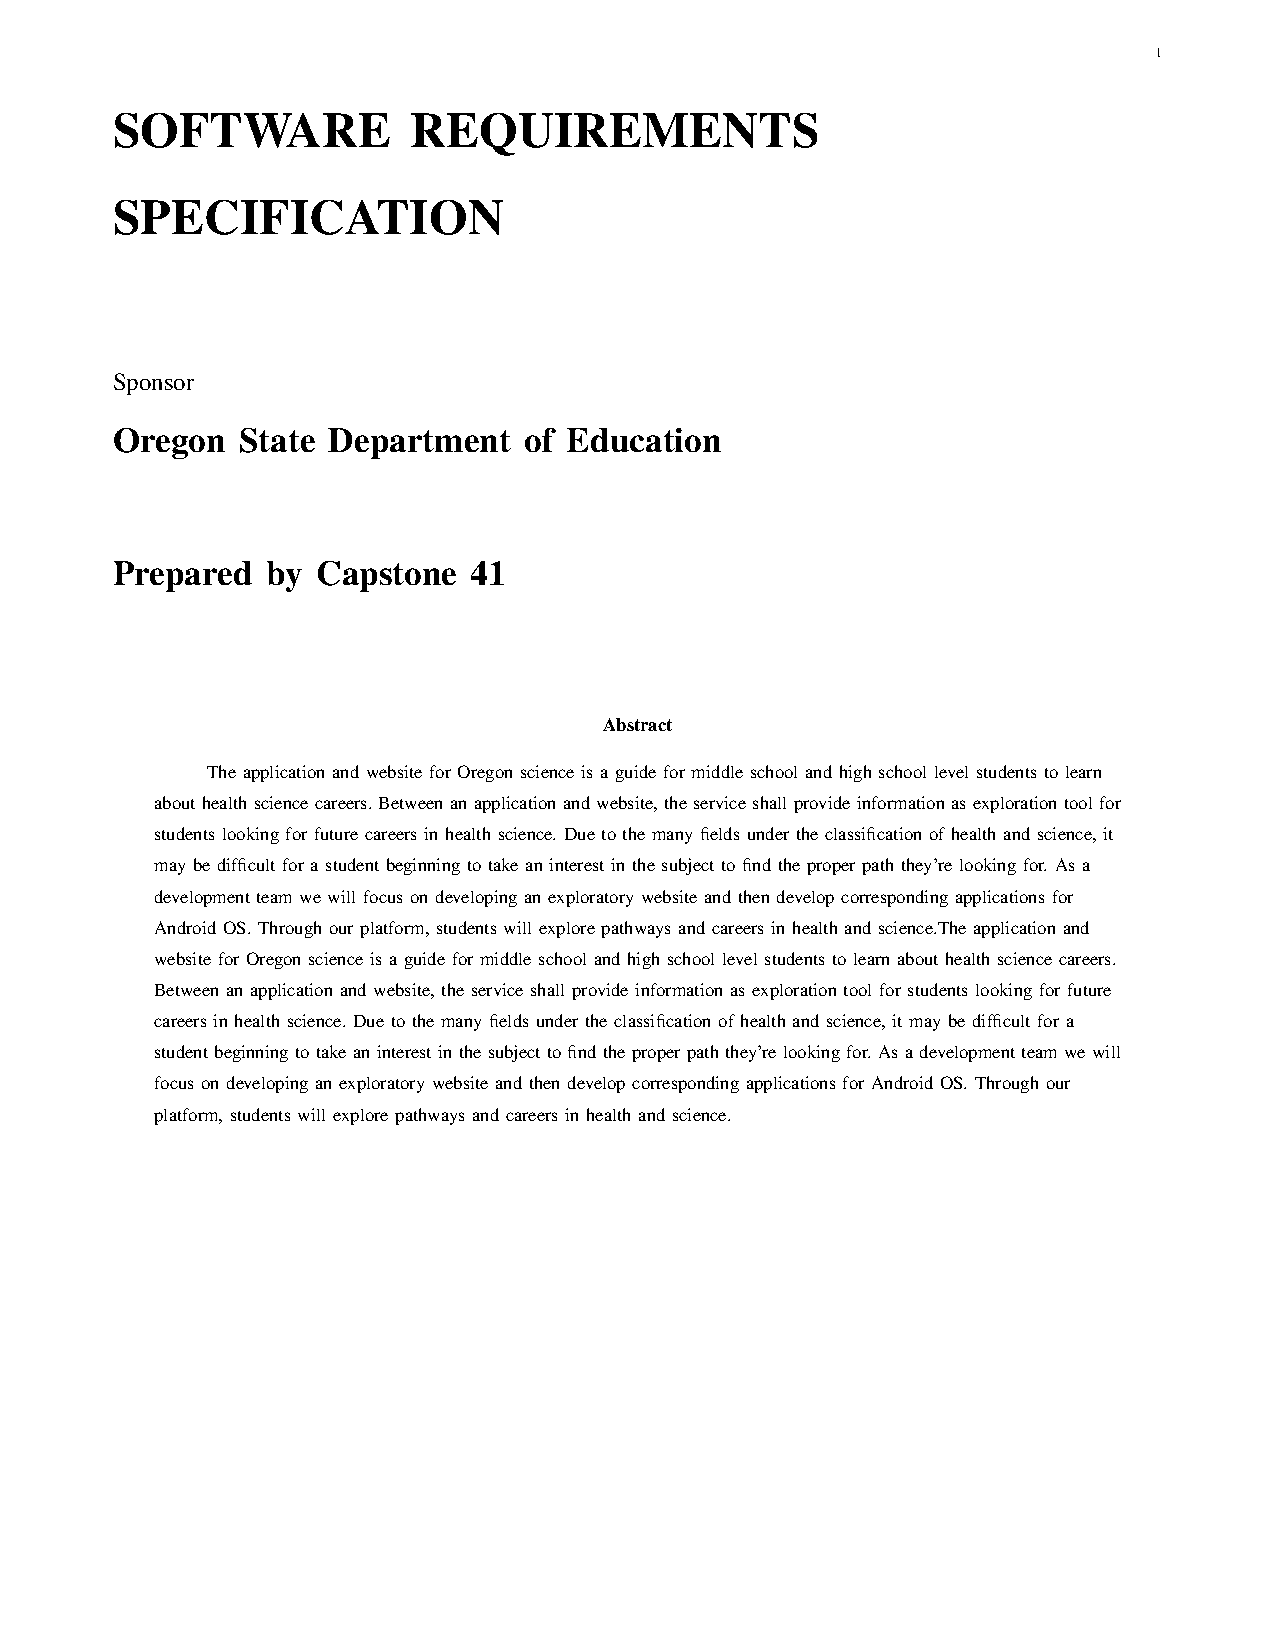
\includepdf[pages=-]{SRS_Final.pdf} 

\subsection{Client Requirements Document Changes}
\begin{center}
\textbf{Requirements Report Chart}
\vspace{0.3cm}

\begin{tabular}
{| p{0.3\linewidth}| p{0.3\linewidth} | p{0.3\linewidth} | p{0.3\linewidth} |}


\hline Requirement&What happened&Comments\\


\hline 
Mobile Application Implementation
&
Changed to single Android Application development
&
iOS application development was pushed to a stretch goal due to foreseen time constraints
\\
\hline



\end{tabular}
\end{center}
\subsection{Gantt Chart Changes}
\noindent Our timeline changed only slightly from our original Gantt chart's planning
\\  \\
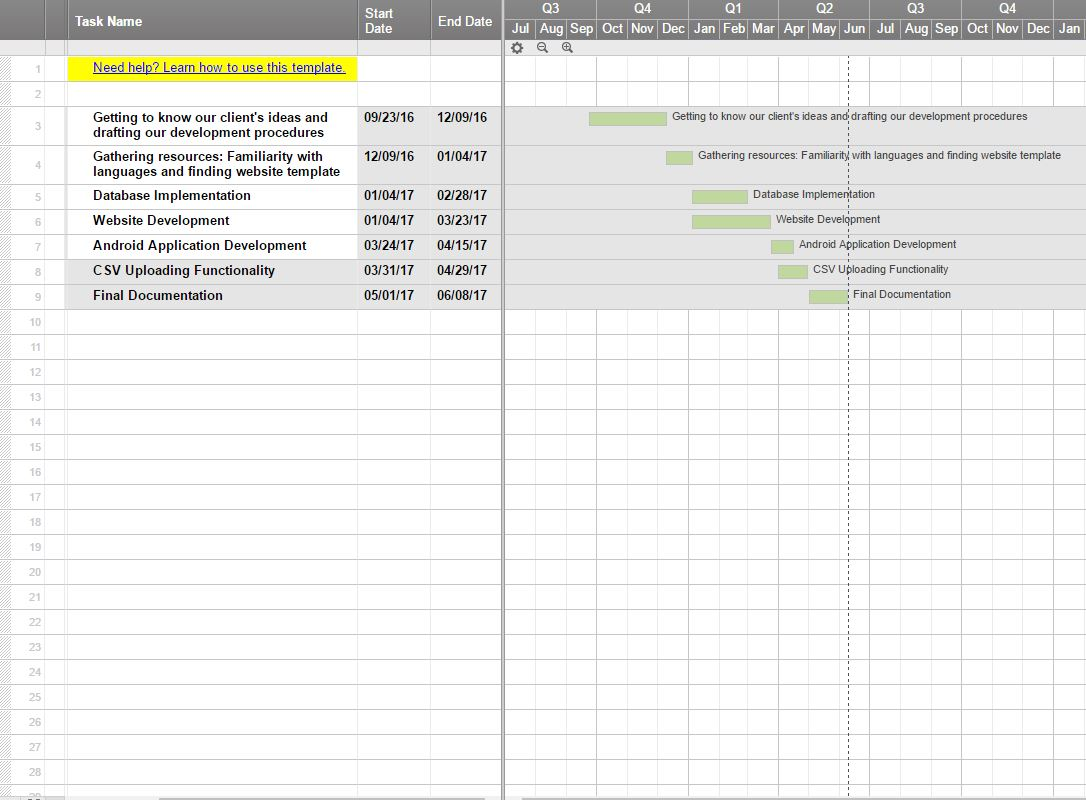
\includegraphics[width=18cm, height=15cm]{Final_Gantt.JPG}
\newpage
\section{Design Document}
\subsection{Original Design Document Draft}
\vspace{2cm}\hspace{2.4cm}
\noindent The following pages include our team's original Design Document.
\\
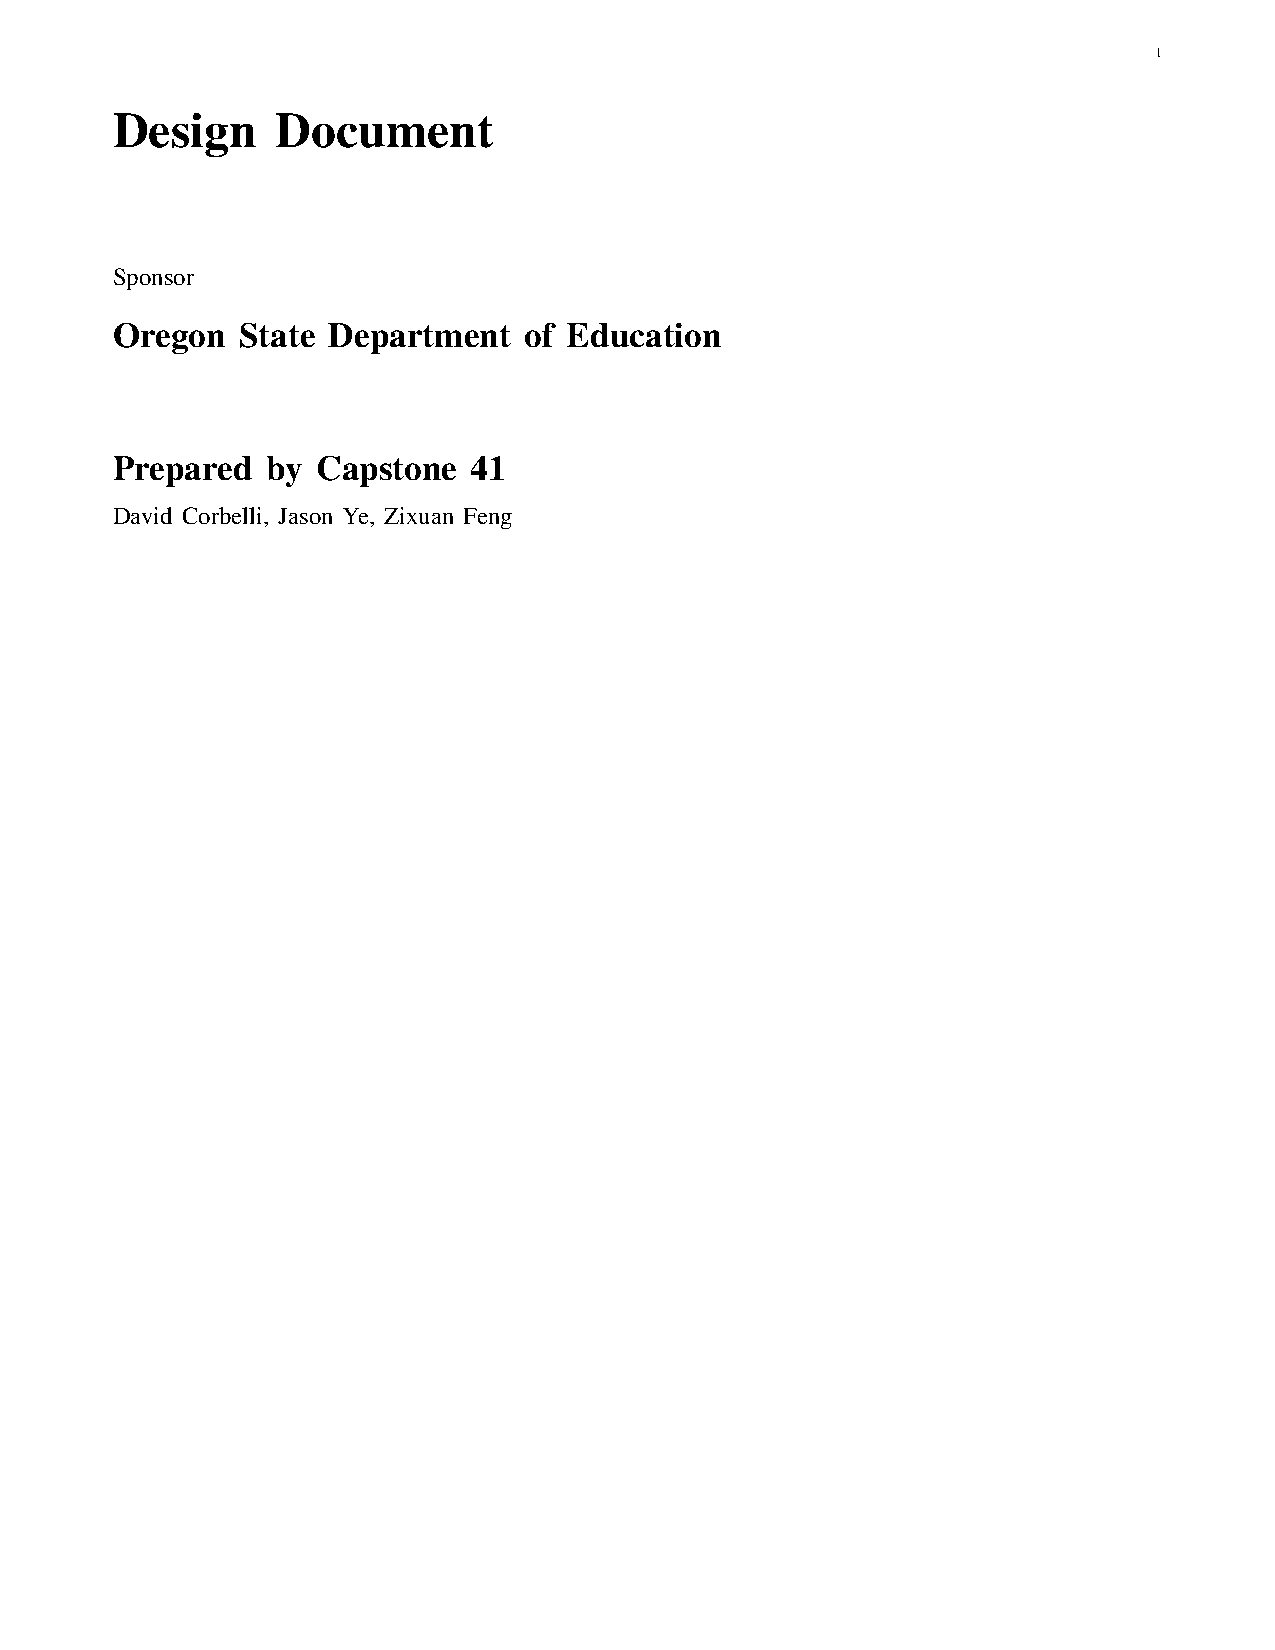
\includepdf[pages=-]{Design_Document_Final.pdf} 
\subsection{Design Document Changes}
\noindent The only change made to the design of our project's implementation was the choice to use a cognitive walkthrough form of user testing rather than the tree testing, click testing, and remote usability testing. This change came about due to the limited functionality of our final website and time constraints towards the end of our project.
\newpage
\section{Technology Review}
\subsection{Technology Review Document}
\vspace{2cm}\hspace{2.4cm}
\noindent The following pages include our team's original technology review documentation.
\\
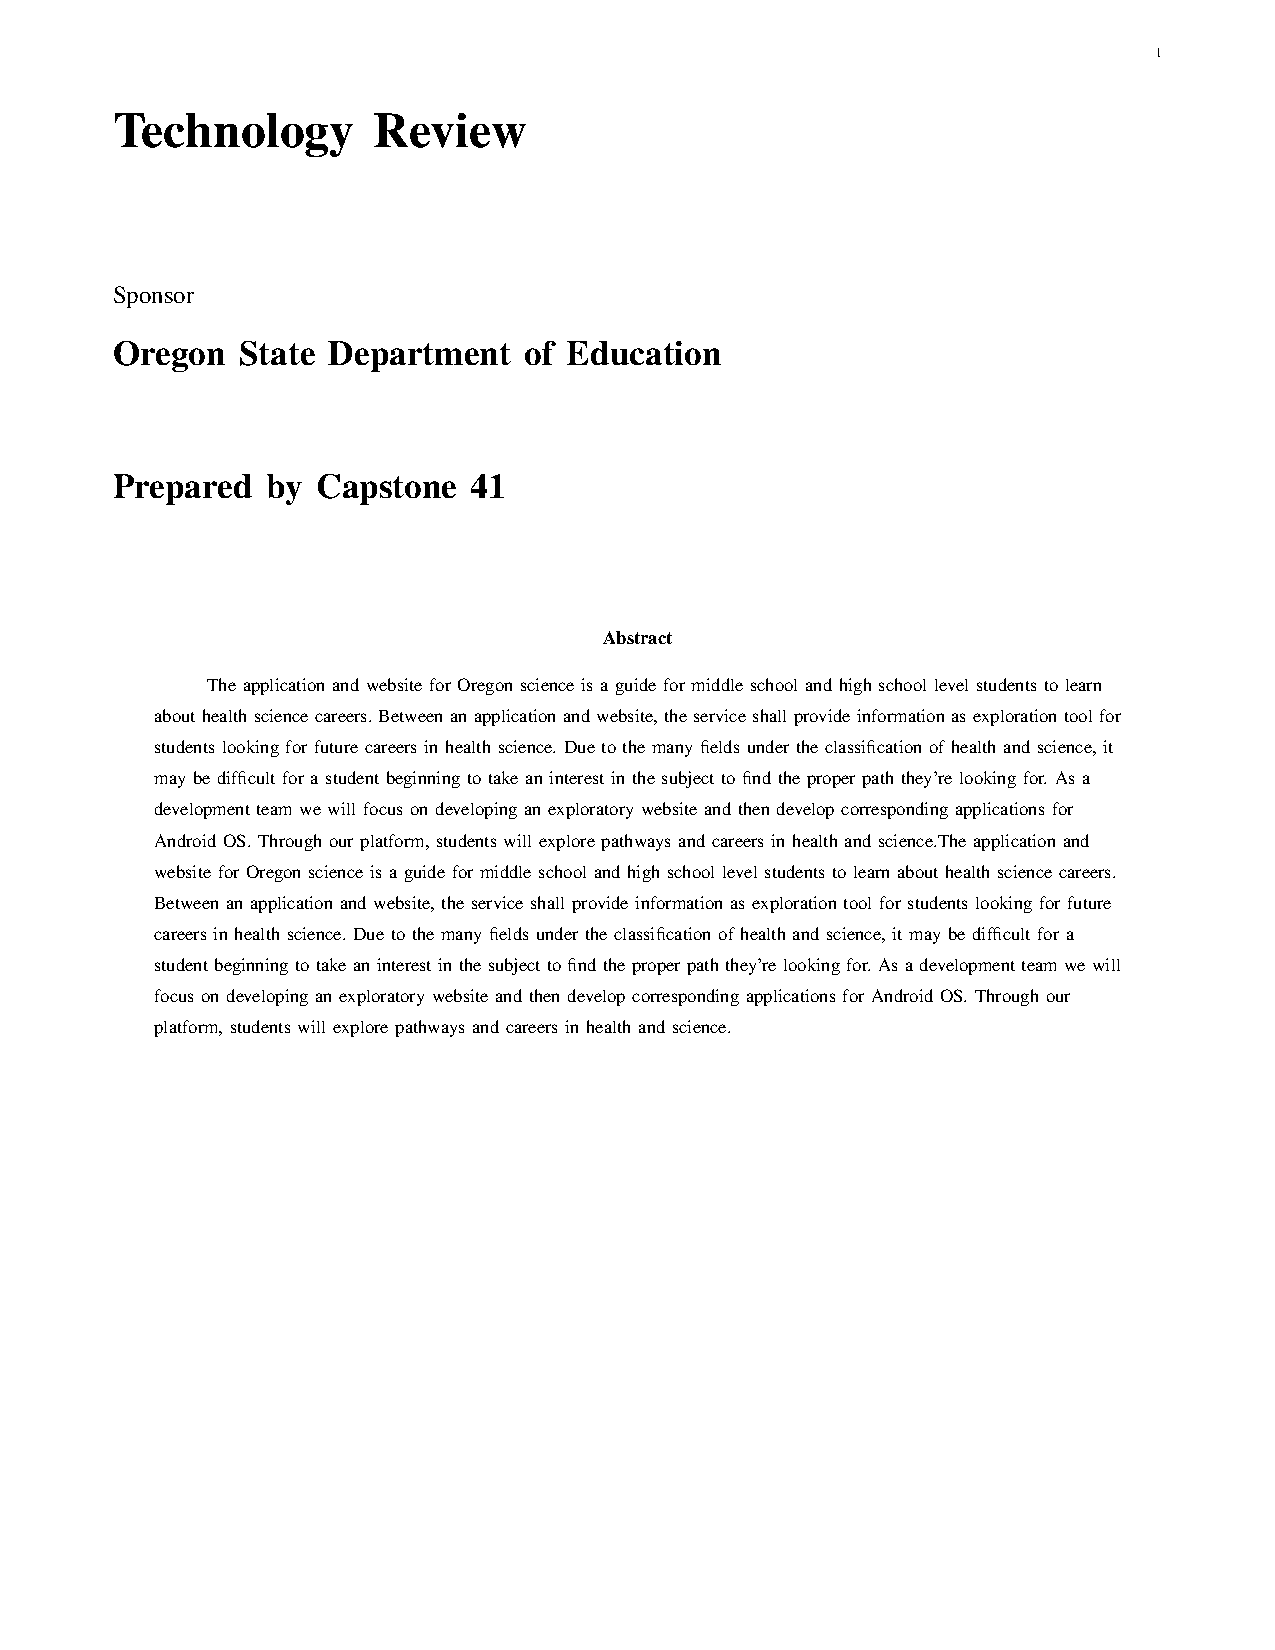
\includepdf[pages=-]{technology-review_final.pdf} 
\subsection{Technology Review Changes}
One major change we had on the technology review is the user testing for the project. Originally, we were planning on using three testing methods: tree testing, click testing, and remote usability testing. On the last phase of our project, we were overwhelmed by the lack of time and limited resources for user testing. In order to test our project effectively and professionally with a small amount of time, we decided to change the test methods into a single user testing called Cognitive Walkthrough, which is a testing process that consisted of gathering feedback and distinguish potential usability problems from users.
\newpage
\section{Team Member Weekly Blog Posts}
\subsection{Fall Term}
\textbf{Week 3}
\\ \textbf{\textit{David Corbelli}}
\noindent As a group we have finished drafting our problem statement document and are awaiting approval and signature. Communication within the group is going smoothly and we haven't hit any road bumps in planning. In testing LaTex seems to have a slight learning curve, but benefits can be seen at first glance. Looking ahead to next week, we will be scheduling an appointment with our TA, John Dodge.
\\ \\
\textbf{\textit{Jason Ye}}
10/13/2016 Last week, on October 5th, we have met with our client through a video conference. My teammates and I have asked about the main objective project. We have talked about the basic functionalities and main focus of the project. Fortunately, Mr.Witkowski is a generous person who enjoy talking with us. He is very passionate about his project and willingly to guide us through every detail of the project. My teammates and I decided to meet with our Mr.Witkowski at least once every week, so we could talk about our progress of the project. We are excited and looking forward working on the project alongside with Mr.Witkowski. This week, we will be turning it a problem statement which define our project's description.\\ \\
\textbf{\textit{Zixuan Feng}}
From Week2, I have met my other two teammate, they are nice and friendly. And On Week 2 Friday, We have a video conference with our cline, Art, he is a kindly person, we talked about this project, what he want get from us, and what is his goal. Through the lecture, we learned a lot from lecture, how to communicate with cline, and how to communicate with teammate. As a computer engineer, communication is one of the most important skill same as the coding. After we talked, we have a very clear mission in the next years. Through a whole week, we have finished our problem statement, including our abstract, problem definition and problem solution, and we sent this to our cline, he is very satisfy with that. On the other hand, through the problem statement assignment, our team deeply know what we are doing and what we are going to do for our cline. And we will talk to our TA next Friday about our project, and talk about our next mission in the future.\\ \\
\textbf{Week 4}
\\ \textbf{\textit{David Corbelli}}
This week we have discussed changes we will make to our initial problem statement submission and have scheduled our meeting times and goals for group work next week. We were also able to meet with our TA, Jon, for introductions.\\ \\
\textbf{\textit{Jason Ye}}
This week, we turnt in the problem statement as a draft and received feedback from the professors. The feedbacks are reasonably simple to fix. Our main focus stayed with our client, and we decided to inform our client about our work through email. In addition, we introduced and met with the TA. Jon, who is our TA, wish to meet with my group and I at least once a week.\\ \\
\textbf{\textit{Zixuan Feng}}
In this week, I reviewed and learned a lot about database and web design tech. Some of them I just learned in this week, and I just reviewed the data tech what i learned before. All these knowledge are prepared for our next step to work on our project. And I watched a lot video about Xcode and Apple Application from Youtube to learn how to develop the IOS application. As for our team, we met our TA to talked about our project and get to know each other. For the next week, We are going to finish our Client Requirement Document, and we begun to start for our website design in next week. We are in a good team, good team-member and great client. We do not have any problem for our relationship. And I still left a lot technology part question for IOS application, I will go solve those questions in next few weeks.\\ \\
\textbf{Week 5}
\\ \textbf{\textit{David Corbelli}}
This week we were able to complete our edits for out problem statement as well and meet up in person to complete our requirements specification. We were also successful in drafting our project time frame. Unfortunately I missed our weekly TA meeting this week.\\ \\
\textbf{\textit{Jason Ye}}
This week, my team and I have met up and worked on the requirement documentation that outlines our project. We have written the necessities and important factors of the project in order for our client to know. We have turnt in the rough draft of the requirement document and hoping for some feedback from our professors. In addition, we have met with John, our TA, and talk about the next upcoming document.\\ \\
\textbf{\textit{Zixuan Feng}}
In this week, We have done the Requirements documents, and we learned how to use the format IEEE Std 830-1998, this is our first time to touch these Latex form, this is hard for us, we did a lot research and spend a lot time to deal with this problem, but finally we finished this task. We just met with Our TA, he is nice TA, and we talked a lot about our Requirements documents, we know we have a lot problems, so we we know what should we do in the next week, firstly, our first step is going to fix the Gantt Graph, we should specific our missions, we should have more than 20 missions. And then in the next coming week, we should learn more about IEEE std 830-1998 ,this is very important for us, we will use this for next whole year.\\ \\
\textbf{Week 6}
\\ \textbf{\textit{David Corbelli}}
This week we worked on editing the format of our software requirements specification document. We worked through several problems in dealing with Latex and were able to conform to the IEEE guidelines. We also met with Jon, who gave us tips regarding the SRS, Gantt chart, and tech review.\\ \\
\textbf{\textit{Jason Ye}}
This week we were suppose to turn in the require document. The document was in IEEE and LaTex format, and we were struggling on making it right. In addition, we could not get our client's signature so we have to turn it in on Monday instead. Overall it was a great experience for us to learn how to do a require document. \\ \\
\textbf{\textit{Zixuan Feng}}
In this week, I learned the real IEEE format for our requirement document. We spent a lot time to fix our privous document. Before today, we still do not know how to use the IEEE format, we do a lot research, and after we talked to our TA, he told us the specific detail, and we fix that thought this afternoon. In the next coming week, we need to do our first individual assignment, it is about the technology, and I will also try to do some research about our IOS application. This is very important for our project.\\ \\
\textbf{Week 7}
\\ \textbf{\textit{David Corbelli}}
Not too much was accomplished this week aside from planning. We made decisions related to the technology review's components. We were able to contact our client to discuss some of our project's direction and have made plans to meet early next week.\\ \\
\textbf{\textit{Jason Ye}}
This week we were assigned a technology review and implementation plan. This document is an individual work which explain what software or hardware needed to be implemented in our project. The purpose of this assignment is to analyze the problem we be will solving and identify the best way to go about solving the problem. In addition, this assignment will help us start our designing process and get ready for program implementation. We were given 9 technology reviews to write about, and total amount of work load is massive.\\ \\
\textbf{\textit{Zixuan Feng}}
In this week, we just finished the document requirement, and our team have worked on this document over 20 hours, this is not a hard assignment, but it is complex, it is a changelle for us, since we need to learn some real programmer's professional skills, not just coding. And by the end of this week, we split the teach work, and we are going to write a report for that in this weekend, this means we have to follow the report and know what part we need to work, and deeply know it and deeply learn it for the project. For the next week, we are going to combine our all the tech report together, and talk about it ,and then be sure every one agree with that, even that is a individual assignment, but it is for our project.\\ \\
\textbf{Week 8}
\\ \textbf{\textit{David Corbelli}}
This week we completed our individual written components and submitted our technology review through GitHub. We also began planning our design document. We have decided to meet early next week in order to ensure we're all on the same page moving forward.\\ \\

\noindent\textbf{\textit{Jason Ye}}
This week we have completed the individual write-up for our technology review. We each had to write up at least 1500 words document which explain what technologies we would be using for our project. The process was a long and tiresome, but it was worth the effort in the end.\\ \\
\textbf{\textit{Zixuan Feng}}
In this week, We finished our tech review on Monday, We combined all our parts together, and formate the document, and write a new abstract for our document. And we set up a plan for our this term biggest document, design document, and we meet with our TA and talk with him about Requirement document and design document. In the next week, since it is a holiday week, we plan to meet our client around Monday or Tuesday, and talk about our client requirement of design document. We still have a question about our website UI, so we need to talk about our UI with client in the next week.\\ \\
\textbf{Week 9}
\\ \textbf{\textit{David Corbelli}}
During week 9 we were able to meet and discuss our project planning through the rest of the term. We were also able to get in contact with our client and decide on a time to conference. The purpose of this meeting will be to discuss visual features of the website.\\ \\
\textbf{\textit{Jason Ye}}
This is week, we prepared to work on the designed document. Its purpose to help us analyze our technologies that we will be using on our project. This document will so help us on the progress report that is due later in the term. It is a holiday week, so we did not meet up with our TA, John, for further clarification.\\ \\
\textbf{\textit{Zixuan Feng}}
In this week, we just set up a appointment with our client to talk about our document design, we set up a plan for our document design, we planed to finish our document during the holiday weekend, and format our design document in the next week. In the week 10, we plan to finish our design document first, and then we will finish our progress report in the next weekend. We only have one problem is the our website UI, so we need to contact with our client to talk bout that.\\ \\
\textbf{Week 10}
\\ \textbf{\textit{David Corbelli}}
This week we were able to meet with our client to discuss various aspects our website. We also finished drafting out design document, progress report, and begin recording our presentation.\\ \\
\textbf{\textit{Jason Ye}}
This week was all about preparing and working on the design document. This document is about writing the step by step of the implementation of our technologies. This document follows the styling guideline from the previous assignment. Overall, it is a brief write-up, and the team and I are working toward the progress report and presentation video.\\ \\
\textbf{\textit{Zixuan Feng}}
In this week, we have finished our design document, and we record our progress report. Basically we have finished all these terms work. We have also discuss the future steps, we will learn our parts deeply and learn the function of boot strap for next term coding.\\ \\
\subsection{Winter Term}
\textbf{Week 1}
\\ \textbf{\textit{David Corbelli:}}
\noindent We received images and information to be necessary for our website from our client. We were also able to share different ideas for website designs to implement
\textbf{\textit{Jason Ye}}
This week is the first week of winter section. David and I have met after class and talked about our schedule. We discussed and mentioned that we needed to meet up a lot more than we used to.\\ \\
\textbf{\textit{Zixuan Feng}}
In the first week, we set up a appointment to meet with each other, and talk about this term's plan, we decided to finish our website in the early of this term, and prepare the application. We planed to start application early in this term since we are not familiar with application, so we need to start our application design earlier. During the break, we have already did some research and ahead work for website, so we could start design right after our meeting.\\ \\
\textbf{Week 2}
\\ \textbf{\textit{David Corbelli}}
missing\\ \\
\textbf{\textit{Jason Ye}}
missing\\ \\
\textbf{\textit{Zixuan Feng}}
In the Week, We have meet with our TA, and talk about our last term grades, we found we did really bad on last assignment during fall term. And then TA we told John about our plan for this term. He agree with our plan, we plan to start the development in week 3. In this week, we have already found some template of website, and did a lot research about Javascript and database. And we have set appointment with our client, we will show him about our website ideal, and talk about the plan with client, if he agree with us, we could start design in week 3.\\ \\
\textbf{Week 3}
\\ \textbf{\textit{David Corbelli}}
We were able to have a long meeting/work period on Wednesday and were able to work out several components of our site. We were able to complete our site's basic styling outline and plan out our database. We intend to work again next week and complete the setup of our database as well as the setup of our webpage's primary component, the career information pages.\\ \\
\textbf{\textit{Jason Ye}}
During this week, we have gathered and worked together on the project. We have received necessary documents and information about the project from our Client, Arts, and started designing the front page of the website. We mainly focus on customizing and arranging the outlook of the website. Also, we began to analyze the database for the site.\\ \\
\textbf{\textit{Zixuan Feng}}
In this week, we just have a meeting with TA and our team again to talk about our progress. We pretty much finished the website frame, so we just need to wait more information and more resources to add in the websites. Our client said we would received the information by next week. So our plan is going to finished the website in two weeks, since we get all the information. Besides, we have not faced any problem seriously. We will have a meeting next week to talk about next progress.\\ \\
\textbf{Week 4}
\\ \textbf{\textit{David Corbelli}}
This week we worked on editing the format of our software requirements specification document. We worked through several problems in dealing with Latex and were able to conform to the IEEE guidelines. We also met with Jon, who gave us tips regarding the SRS, Gantt chart, and tech review.\\ \\
\textbf{\textit{Jason Ye}}
This week I went to class for the third time of this term. Class discussion was about the upcoming progress report, Alpha stage of the project, and more in dept of the Expo. Also, the team have met up and worked on the database for the project. We have gotten most of the schema done, but we still needed to input the information into the database. \\ \\
\textbf{\textit{Zixuan Feng}}
In this week, we tried to contact with our client and get more information for the website, but we only got the branch of the websites, we might need to re do our website database. otherwise, we have not received any more information from our client, so we plan to continue to design our application next week. We assigned our different task to look up and search some frame of our mobile applications.\\ \\
\textbf{Week 5}
\\ \textbf{\textit{David Corbelli}}
This past week we were able to discuss certain visual features of our website and begin the process of writing our winter progress report using Overleaf. We received certain documents from out client related to webpage mapping, but are still waiting to receive content for each webpage. We're working to meet our deadlines, but we feel slightly behind. We have decided it may be best to shift focus towards our web app development rather than waiting for the completion of database components\\ \\
\textbf{\textit{Jason Ye}}
We went to class and received important information about the upcoming progress report and OneNote. These tasks are meant to be keep track of our project timeline. In addition, we have email to our client, Arts, on receiving more information about the website. The upcoming week will be very busy for each of us.\\ \\
\textbf{\textit{Zixuan Feng}}
In this week, we still have not received more information from client, we still working on our website database, and planning our mobile application. Currently, we decided the mobile application as the mobile cite application, which is good for our application purpose. This app should be small since it is only a small application should be only contain the introduction of career, if the application is too complex, we sill not have too many customers. And we are working on our progress report, we will try to finish that before the due date, we could let our TA to help us check that. Next week, we will still working on website and we try to finish that before the week 8.\\ \\
\textbf{Week 6}
\\ \textbf{\textit{David Corbelli}}
This week we spent time developing our website as well as completing course documents. We were able to import data into our database as well as setup the career information page using PHP. We spend the next two days working through our progress report document and recording our video\\ \\

\noindent\textbf{\textit{Jason Ye}}
This week, we have met up and worked on the project significantly. We completed the Alpha state of the website which would be presented to the professor. We have also worked and completed the progress report which is about the progress of our project so far. We made a video with powerpoint slides related to the progress report. We still have a lot of things to work on and discussed upon, so we will continue to work on the project for the upcoming weeks.\\ \\
\textbf{\textit{Zixuan Feng}}
In this week, we finally received information and data from out client, he gave us a new spreadsheet, and we used the new spreadsheet to fix our database again. Because the previous spreadsheet is too complex, it is not good for database setting. And we finished our website framework as well. We only left put more data into website. Other wise we finished our website. Next step, we are planning to start our mobile application, we want to polish our website in next week, and finish our mobile application frame by the end of the term.\\ \\
\textbf{Week 7}
\\ \textbf{\textit{David Corbelli}}
missing\\ \\
\textbf{\textit{Jason Ye}}
This week we have met up together and worked on some more on the project. We have figured out the framework of how the website display the information of careers. To display the information more efficiently, we had to think of a way to have a page where it stores and shows all the careers. In addition, we have met up with our TA after 2 weeks due to his sickness. We have talked about the upcoming assignments and EXPO date.\\ \\
\textbf{\textit{Zixuan Feng}}
In this week, we meet to finish our website. Last week, we finish the database for the website. So we only left to add more pages for website and polish the website. So in this week, we add two more pages for career. We tried many ways to design the career, since there are a lot information of careers, it is hard to organized, we decide to use a chart to list the career and information of careers. We are a little bit behind of our project, so we plan to start the application in next week, at least we could have a general plan for application. We just talk with TA this week, he said we still have one more month for app development in next term. We assign the missions for this weekend to find a tool to develop application of android besides google engine.\\ \\
\textbf{Week 8}
\\ \textbf{\textit{David Corbelli}}
This week I attempted to get in touch with our client. We're putting the finishing touches on our desktop website, but we are still behind in our progress. By Sunday, I intend to have finished styling the career information pages, Zixuan will have finished styling the career navigation page, and Jason will finish styling the image component of the home page as well as integrating web analytics. We still need information relating to the remaining home, about, contact, external resources as well as many of the health careers themselves. We aren't quite sure of Art's agenda, but I am worried about our timeframe. We intend to begin development on our web app next week.\\ \\
\textbf{\textit{Jason Ye}}
This we have polishing up the website with the limited information. By finishing up the website, we will able to get started on the web and phone application. We have done some research on how to implement the web application as far as learning how to coordinate the web and phone app.\\ \\
\textbf{\textit{Zixuan Feng}}
In this week, we finish the database and we finished most part of our styling. I worked on the career's page and i did some styling work for every chart in the page. Besides, we are planning work on mobile cite in the next week, we planned to finish the mobile cite before the end of term, then we will have time to finish our android app by the expo.\\ \\
\textbf{Week 9}
\\ \textbf{\textit{David Corbelli}}
This week we were able to make progress towards our web application and Android app. Zixuan was able to setup Android Studio and I was able to find an application template to create an abstracted web browser view port. We had planned to move on to this step to test our in-progress web application. Jason also began to work towards an PHP page to upload CSV files to our database.\\ \\
\textbf{\textit{Jason Ye}}
This week we have accomplished a lot of necessary tasks for the project. First, we figured out how to convert the desktop site into a web app. Steve has found a lot of information about the implementation, and he has been working to the point of completion. Next, we used a temple guideline to create a mobile application referencing to the desktop site. It went very well in terms of technological and logical sense. Finally, I have implemented a way for our client to input information into a Excel sheet and upload it to the database and display it on the website.\\ \\
\textbf{\textit{Zixuan Feng}}
In this week, we worked on the our mobile applications, since we almost finish our websites. I finished a mobile website template, but it is not our team asked for, so i just put my work back to shelf as a plan B in the future. We downloaded a template for android studio, this is a template and framework for us to put our website and transfer into mobile application. What we left is only some styling, but the bootstrap also provide CSS package for us to edit the styling for shirking. And we done with some pages, but we still left some pages. In the next week, we are going to finish the poster draft 1, and we set up a meeting with our client on Monday to talk about our website, and finish the progress report and presentation.\\ \\
\textbf{Week 10}
\\ \textbf{\textit{David Corbelli}}
We spent this week wrapping up development for the term and figuring out what requirements we have left to implement and also conversed with our client regarding domain hosting. We also spent time writing out our progress reports and recording the video progress report.\\ \\
\textbf{\textit{Jason Ye}}
This week is a dead week and we have had so much accomplished on the project. On Monday, we have had a video conference with our client. We have showed him the beta stage our the website and the mobile application. In addition, we have asked for an in-depth version of a csv file containing health careers. Our client has shown great joy after seeing our result and he was happy about the project. Furthermore in the week, we have met with our TA for the last time for this term, and we talked about the upcoming EXPO event.\\ \\
\textbf{\textit{Zixuan Feng}}
This is the last week of this term, since we have already done our project for eighty percent. And we met our client in this week, and he is very satisfied with our current products, and we asked more information and requirement documents we need for next step database building. In the next term, we plan to finish the rest of part before week 3. We have not left any problem in this term, everything is in order.\\ \\

\subsection{Spring Term}
\textbf{Week 1}
\\ \textbf{\textit{David Corbelli:}}
\noindent Our plans for this week had included meeting up again in order to regroup and discuss what tasks were left to complete within the last month of our primary development.Over spring break we were able to receive an updated spreadsheet to include data for several more career paths. Coming back from spring break, very little development had occurred since our previous progress support, but we had begun to look into CSV uploading to interface with our database.No problems were met during this week.
\\ \\
\textbf{\textit{Jason Ye}}
Starting off this spring term, we have went to class and learned more about the upcoming event that is near. Since it is coming up so soon, we have got to prepare for it. Also, the teammates and I haven't heard from our client yet, so we are kind of stuck in the process of delivering the full content of the project. Overall, we are preparing for Expo.\\ \\
\textbf{\textit{Zixuan Feng}}
In the week1, we meet with our TA and we talk about the next progress, and we set up an undo list, and we separate the work for this term. After that, we did some changes for our websites interface and we fix some problem for the database. For the next week, we are going to finish the poster draft 2 and try to polish our website and database.\\ \\
\textbf{Week 2}
\\ \textbf{\textit{David Corbelli}}
Our only plans for this week included further development of our website and taking time to look over our poster draft.Over the course of the week Jason took time to further develop the CSV uploading PHP pages, while Zixuan and I made progress finalizing our Android Application. I implemented the domain name hosting and we were able to get the native application interfacing properly with our web application.We emailed Art the previous week asking about database hosting solutions, but have not gotten a response.\\ \\
\textbf{\textit{Jason Ye}}
This week, we have met up with our TA, Jon, to talk about and schedule our new weekly meet. Jon mentioned about the registration for Expo and more in-depth of Expo day. Also, we have met up two times and worked more on the project in terms of finishing up the requirement and polishing the technology.\\ \\
\textbf{\textit{Zixuan Feng}}
In the week 2, we finish our poster draft based on the OSU poster requirements. And then we polish more UI staffs for the websites, we do not need to worry about the applications, so we just focusing on the website. And we separate the database works, i am in charging of email part, i tried very hard, but i still need to fix some development in the next week\\ \\
\textbf{Week 3}
\\ \textbf{\textit{David Corbelli}}
This week our plan was to wrap up the majority of our development for the impending code freeze and finalize our poster draft.Jason had a nearly working implementation of the CSV upload pages completed, while I had gotten the code necessary to generate PHP webpages for all input careers nearly working. Steve worked further on our project's documentation. As a group we were able to finish our poster draft and send it off to our client.We have still not heard back about the databases nor about our poster's approval.\\ \\
\textbf{\textit{Jason Ye}}
This week we have met up with Jon to talk more about the final progress of the project. We talked about how we going to present it on Expo. In addition, we took a team picture to be posted on the poster draft. One major problem we are still having is the issue of contacting with our client, Art Witkowski. David and I have emailed and called him during daytime, but we have not heard from him.\\ \\
\textbf{\textit{Zixuan Feng}}
In this week, we have done our final vision of our poster, this is the biggest thing. And we sent to our client, but we have lost connection with our client since this term start, i do not know if we could get the response in the next week. And I finish the email part of our website, basiclly it could allow the user send email from the webiste to adminstrater. Since our code is due on next Sunday, so in the next week, we are going to polish our programming part, and coding part. Otherwise, we only left the report and documentation to do in the rest of term.\\ \\
\textbf{Week 4}
\\ \textbf{\textit{David Corbelli}}
This week our plan had been to wrap everything up and get things uploaded to Github. Jason had a working version of all pages except career deletion from our database, and I was able to implement the generation of webpages without much difficulty. Other modifications included validating all navigation worked as intended and we also finished our user testing. I took the time to delete unnecessary files from Github and organize our repository.We still have not heard back from our client since spring break despite several phone calls.\\ \\
\textbf{\textit{Jason Ye}}
This week we are hoping to contact with our client one last time. Due to the deadline of approving our poster, we needed to get in touch with Art as soon as possible. Our last resort is to talk to our professors about our issue. Unfortunately, Art have not contact us; we haven't talked to him for 4 weeks. It was a huge concern for us and we were trying our best to complete and meet all the requirement of the project. We have met up with another team to analyze each other poster for addition credits. Also, we have met up a few times to finish up and upload the project onto Github.\\ \\
\textbf{\textit{Zixuan Feng}}
We have lost communication with our client since beginning of this term, we have not received anything from him. But we are still moving forward, we are using what we got, like OSU server, OSU database, etc. We have already talked with our professor the current situation, he said he will be our client if we cannot get anything from our client by the end of this term. We have done most of thing we need, rest of weeks we only left the manneal and polish our website for one more time. We did not left any problem. We will continue working on our EXPO in next week.\\ \\
\textbf{Week 5}
\\ \textbf{\textit{David Corbelli}}
We had little planned this week except for preparing for expo.
I was able to compile all of our documents and push everything to Github on Monday and Art responded to my email replying that he would get in touch with his IT department for database setup.
No problems occurred during this week.\\ \\
\textbf{\textit{Jason Ye}}
On Monday of this week, we have submitted the final phase of the project to GitHub. All of the codes and paper work are successfully submitted for grading purposes. In addition to this week, we have met with our TA and discussed more about the Expo event and poster. Fortunately, our client, Art, have finally responded to our email. After four weeks of unresponsive contact with my team, he replied with messages about providing the database server to us. We still are not sure about his future connections with us but hopefully he will stay in touch with us more.\\ \\
\textbf{\textit{Zixuan Feng}}
In this week, firstly, we finished the final draft our poster, and we polished our website, since the MAY 1st in the last day for upgrate the programming part. On Friday, we set up a meeting with another group to do the peer review poster, and we are confident with our poster right now after a little bix fixing. In the next week, besides the programming, we will begun to move forward of the adminsteration book for our client. We still have not received any infomration from our client. We will still move forward.\\ \\
\textbf{Week 6}
\\ \textbf{\textit{David Corbelli}}
Our plans this week included preparing our progress report and our presentation for expo. We had planned to meet on Friday to conduct the majority of our recordings, but only two of us were able to meet.Not much development occurred this week except for the preparation of our slides and script for our video presentation. Zixuan and I were able to record the majority of our speaking sections for the progress report video.Art still has not contacted me about finding a database solution.\\ \\

\noindent\textbf{\textit{Jason Ye}}
This week, we have completed our requirements for the project, and it is ready for Expo. David have emailed our client about our Expo and fortunately we have heard from him for the first time in a very long time. Art was kindly replied about not able to make it to the event due to his busy schedule. So far, our concern is to make sure to complete Expo without any issue. Our TA, John, was not available for this week meeting. Instead, we used time to talk over the Expo procedures and scripts.\\ \\
\textbf{\textit{Zixuan Feng}}
In this week, we have finished everything we required and we still have not received any information from our client. We checked our design document and other files, we have meets all the requirements and designing. There is nothing left for programming development. We are preparing the EXPO presentation and progress report. We trying to make a appointment with professor Winter to see if she could help us to give us some advices and suggestions for EXPO presentation. We will continue preparing for next week EXPO, and keep running and testing our products to make sure no bugs or bad things happened during EXPO.\\ \\
\textbf{Week 7}
\\ \textbf{\textit{David Corbelli}}
On Monday we planned to meet in order to record the remainder of our presentation and on Wednesday had planned to meet with Winters about devising our expo presentation.We meet early on Monday to conduct the remainder of our recordings, finalize our slides, and write our progress report. That evening I edited the video and submitted everything through email and GitHub. Our discussion with Winters was productive as we were able to determine what worked well in presenting and things to keep in mind.The Engineering Expo on Friday went well for our group. We didn't speak to many visitors, but it was a good experience and were prepared to answer the questions that were asked.Art contacted me this week to notify me that he does not currently have access to a database nor funds prepared to set one up.\\ \\
\textbf{\textit{Jason Ye}}
This week we have prepared and wrote the script for the Expo presentation. We wanted to make sure that each of us present the same idea to our audiences. In addition, we have talked to TA and talk about the final preparation for Expo. Expo day went well as we have imagined and we were very proud of each other. Each of us checked in at 8am and ended our presentation at 3:30pm.\\ \\
\textbf{\textit{Zixuan Feng}}
In this week, we focusing on the EXPO show on Friday. We prepared a lot, and talk with Professor Winters and TA John about some suggestions and advices. After combined the suggestions and advices, we arranged our expo time slot and we could switch our position and take a rest. Finally we had a very smoothly and successful EXPO show. And we accepted about 30 people and talk about our project. In the next week, we need to do more things about document and begun to prepare the manual for our client.\\ \\
\textbf{Week 8}
\\ \textbf{\textit{David Corbelli}}
We had not setup any plans for working this week. We still, however, need to finalize our project's documentation and begin our final reports. I will contact our client about the handoff of deliverables as well.Project progress was not accomplished this week.No problems were met.If i were to redo the project from the start I would tell myself to start earlier and ask more specifically for what we require to develop the website and request a deadline for its availability.The biggest skill I've learned is group management and time allocation from this project. The skills I can see myself using moving forward include certain management skills and web development.I liked certain freedoms we were given in our development, however, we learned this freedom requires more responsibility and diligence without our client watching over our shoulders.I from my teammates how to work as a team. We were able to split up tasks efficiently and put together a final product we were all satisfied with.If I had been our client, I believe I would be satisfied with our group's work, however, greater stakeholder input might have expedited and improved the final product.If any continuations were to be made to this product they would most certainly be in the area of webpage styling and functionality. There are many areas of this website currently only holding placeholder data and paragraphs; once these are filled in there will be room to perfect the styling of the website and add to the content available.\\ \\
\textbf{\textit{Jason Ye}}
After the Expo event, we have met up in class and with my TA to talk about the final assignments regarding to Expo. We were assigned with a couple of tasks about the Expo and the overall year experiences. During the TA meeting, my teammates and I talked about the general thoughts about the Expo. We briefly mentioned some personal thoughts and ideas about the Expo. After the meeting, we have decided to meet up as a team and work on the user guide manual for our client and ourselves. As for the client review for our Expo, we still have not heard from him. Part of our grade is based on his review, and we are hoping to hear from him as soon as possible. If we do not hear from our client, Dr.Winters or Kevin will be replacing our client and become our main grader instead.This project was fairly easy and reasonable for all of us to complete. If I was to redo the project, the one thing I would do is to implement better features and user interfaces for our target audiences. In addition, polish it with better CSS styling. The number one skill I have developed and learned over the past few weeks is the implementation of uploading data into the database using various file type. I feel that it is a essential skill to have for my future job. This project has taught me a lot of things I have lacked on, and I enjoy working on it. Web development has always been my passion and I did not regret working on it with people I trust. The one thing I do not like about this project is the lack of communication with my client. If we have spoken more about the project, I would have worked and learned more on it. As a team member, I have learned so much important aspect of web programming and database management from both of my team members. They have corrected and taught me many skills that I lack on. If I was the client of this project, the number one thing I would do is to keep in touch with the workers as many times as possible. Having well-instructed and constant communication is very important for completing the project. If this project were to be continued next year, I would work on publishing the web pages and implement more user interface.\\ \\
\textbf{\textit{Zixuan Feng}}
In the past week, we had a class meeting and cheer our EXPO last week, and we met our TA on Thursday to talk about future documentation. During the meeting with team members, we talked bout last week EXPO, and exchange our thoughts and ideas. And We made a plan for future missions. We planed to meet on Tuesday next week to finish our manual for our client for future administration. The only problem we met is we still have not received our client any ideas or feedback for our project, but we will still finish our project entirely. TA said if our client will not contact us anymore, our professor would pretend our client and grade our project. If I would redo the project from the fall term, I would tell myself contact with our client tightly, and maybe go to Portland to meet with him. And I would tell myself pay attention at database, this is the main function of our website. The biggest skill for me I learned how to use the Android Studio to develop a web app, before this class, I have not touched the Android Studio and Java yet. This project provided me a good chance to learn the Android Studio and Java. For me, I think if I could work in some website company, database will be my majority work and if I do the UI design for some websites, CSS and HTML would be my majority language to explore in the future. I like our project, because it is a classic computer science works, and if I go out for work as a bachelor degree student, my job could be same as our project, and this project bring me to the real computer science world and work. I do not have anything dislike about our project. Firstly, I learned how communication skills from our team leader David corbelli. He is in charge of contacting with our client, and his methods are professional and I learned database skills from my teammates Jason Ye, he is good at database skills. If I could be our client, I am satisfied with our project, we not only finish our project completely and entirely, and we also created some ways to make the website easier to manage in the future for our client, this is not requirements, we did a lot extra works for our project, these works not only face our requirement, but also give client extra help to manage website and application. If we need to continued to work on our project, we will continue to develop a IOS application, and publish both IOS and Android applications, and maybe make more pages or more functions for our website, We could add a user log in and register function, and we could more pay attention at user’ interaction.\\ \\
\newpage
\section{Final Poster}
\vspace{2cm}\hspace{2.4cm}
\noindent The following page includes our team's Engineering Capstone Expo poster.
\\
\newpage
\section{Project Documentation}
\subsection{Usage and Maintenance Guide}
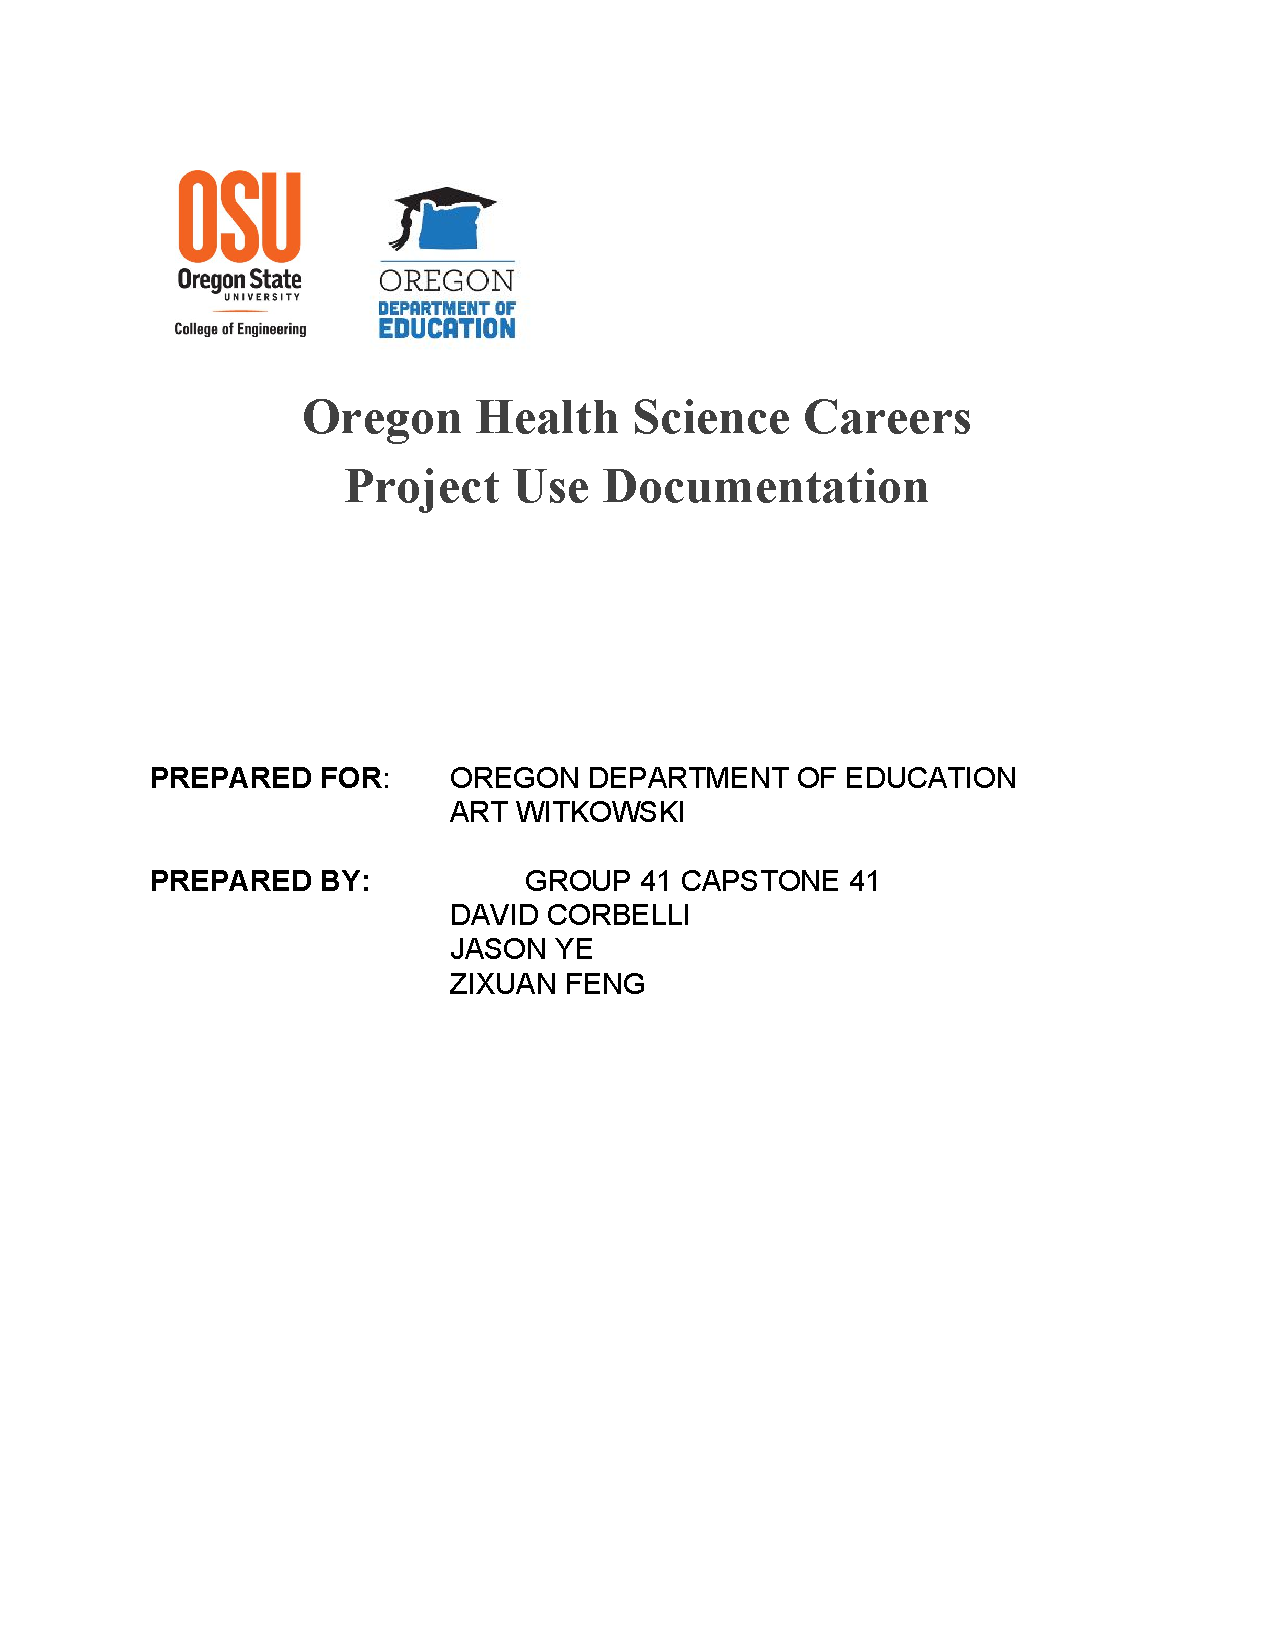
\includepdf[pages=-]{WebsiteMaintenanceManual.pdf}
\subsection{Mobile Application Installation}
\noindent In order to install and run our Android application is necessary that the user download and run our app's .apk file from our GitHub repository at:  https:\/\/github.com\/corbelld\/EECS\_Capstone\_Group\_41\_2016\-2017.
\subsection{Theory of Operation}
\noindent In theory, our website or application will be used by middle and high school students looking to gain information about a career path in health sciences. They will begin by visiting our website's homepage and then will likely move on to visit our careers navigation page through our intuitive navigation bar. From here they will access the career information page they find most appealing and repeat this process until sufficient knowledge is gained or their interest is satisfied. 

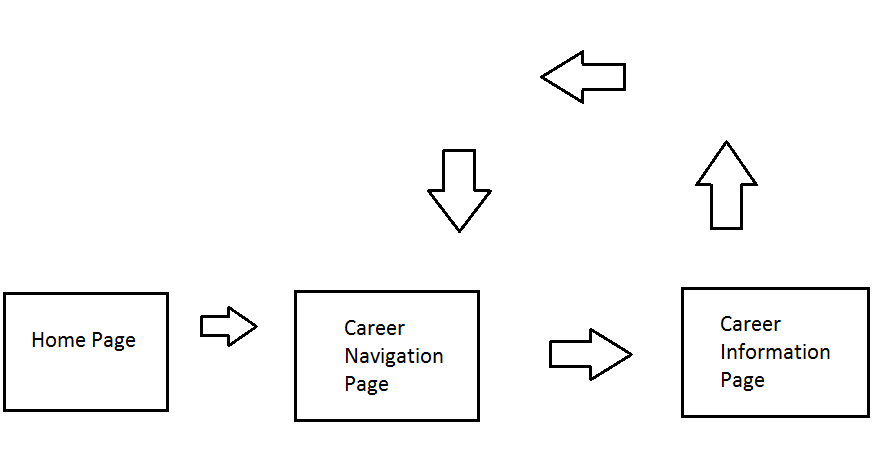
\includegraphics[width=16cm, height=8.8cm]{doc11.png}
\newpage

\section{Learned Technology}
\subsection{New Technologies}
\noindent The majority of the information our group learned was gained through online research. 
Several of the skills we learned include certain PHP functions used to read-in and process CSV spreadsheet files, SQL code for database construction, CSS code for styling implementation, and the use of Android Studio for mobile application development.
\\ 

\noindent For the PHP functions we looked through similar implementations posted online and took time to deconstruct the processes being used. Through reviewing this code as well as W3Schools' PHP documentation we were able to understand and implement this technology.
\\ 

\noindent Documentation available through W3Schools also aided us in our SQL implementation. We use SQL queries for a variety of tasks including information validation, database updating, database deletion, and for drawing information from the database. In order to ensure we used these queries properly required certain review of the online site. 
\\ 

\noindent Our CSS styling, implemented using Bootstrap required research into the usage of Bootstrap's styling framework. Sites referenced include Bootstrap's homepage, which contains in-depth documentation of the majority of Bootstrap's native features, as well as certain blogs detailing additional usage, which can be derived from the original implementation. Aside from Bootstrap we also used W3Schools again for more basic CSS knowledge and for styling changes desired specifically for our website.\\

\subsection{Useful References}
\noindent Recalling the development process we did, we think there are amounts of books and websites helped us. Before we created this website, researching was always playing a significant role, since we are only senior students, most of the technology related to real website development were still strange for us. As for my part, we used following website to helped me learn the basic website designing:
W3C school helped us learned the HTML, PHP and CSS works. 
The “developer. Android. Com” (official android studio website) helped us learn the android application development. 
The “Mysql.com” helped us learn the MySQL and database skills.
“GitHub” always plays a library role during our development, there a lot open source library we could use for references.
Since before the project, we all have never touched the android application before, we also used a book to use as a reference, “Android Studio Application Development”. 
In order to list all the website and books, we would rank them in order of helpfulness:
“GitHub.com”, “W3Cschool.com”, “developer.Android.com”, “Mysql.com” “Android Studio Application Development”.
As for people in the campus, we think the previous professor gave our a lot helps. sent several emails about CSS and HTML question to our previous professors. Most of professors are very friendly and willing to accepting questions. \\
\noindent Other useful sources during the process of working on website were looking at existing websites that dedicates to health science career pathways.
The websites was based on a specific region which helps and guide students to explore current pathways and health science careers.
In addition to using third party websites, we have looked into website templates that would help us create a user friendly site.
Our focus was that the website needs to be user friendly, organized, clean and easy to use. 
A template we decided to use was a bootstrap theme from startbootstrap.com. The template’s theme was business casual and had met all of our desired requirements.
The web site was very helpful for starting off of our project. 
Another useful guide was a website we used as a reference for importing spreadsheet with data into the database. 
The website, CODEXWORLD.com, give us “baby step” of how to import CSV file data into MySQL database using PHP.
In the site, the helper provided a video along with step-by-step procedures. \\





\newpage
\section{Individual Learning}
\subsection{David Corbelli}
\noindent Through the capstone process I was able to gain knowledge and experience, both technical and non-technical. Technical aspects of my learning include greater familiarity with PHP, HTML, CSS, SQL, relational database structure, and experience with the use of Android Studio. While I had had experience working with many of these technologies at a basic level through my CS classes, this is the first time that a project was given to me without initial requirements as to what functions or technologies needed to be used or implemented. The use of many of these languages and technologies and to what end they were used were decided by our group and we gained much greater familiarity with each by the end of our development.
\\ \\
Learning in non-technical areas came large in-part from the need to work and communicate with a team. With the three of us having different levels of experience with different technologies going into this project, it became necessary for us all to stand at at a shared level of understanding for each component of our website before we could proceed. This project also gave me my first opportunity working and communicating with a client. While I've worked retail and have had customers before, this is my first time working with a stakeholder to complete a project with a vision devised by a second-party. It was often that our group would ask questions, but not fully understand our client's desires and we would need further clarification. From this I learned how crucial it is to formulate a plan and think through questions before hand as to not waste or clients or our developers' time.
\\ \\
Working on a long-term project was a new experience for me. I had never previously worked towards any single product for as long as we developed this website. I was able to learn about work-flow and how the simultaneous development of different components can come together into a functioning final product. It certainly would have been difficult to accomplish what we did alone and I learned the necessity of having a team.
\\ \\
Through this project I was able to gain leadership skills as well as a greater sense of time management. Over the course of the year it was often one of my responsibilities to devise what are team would be working towards at each of our group meetings. Because of this, it was often part of my job to maintain a sense of how much work was ahead of us before our next due date and ensure we were able to each work on a remainder of the project in an efficient manner. I learned that it's necessary to formulate a strong plan early on in development and seek out all requirements towards development before the implementation is needed. 
\\ \\
About working in teams, I learned that it's necessary to have strong communication of ideas. It is of utmost necessity for all members to be on the same page before implementing separate functions; in the cases that we did not all have the same vision in mind we lost time developing several functional components of the website. Furthermore, it's not always important whose idea gets used as long as the work gets completed in a timely manner. 
\\ \\
If I were to redo this project differently, I would consider pouring much more work into the early planning process of the project and gain a clear vision of the client's vision, expectations, and available resources. The ability to keep all of these in mind from the start would have kept us from needing to halt development while waiting for answers. I believe that doing a better job of this early on might have allowed us to complete this project to a greater degree.

\subsection{Zixuan Feng}
\noindent As for me, I learned a lot from this whole year. 
Technical information: Before I attended this project, I have never attach the bootstrap, I learned how to use bootstrap to set up the website frameworks. As for mobile application, I have never learned Language Java before, but I learned from different website to know how to set up the android application by using android studio. We used a open source android application program as a references and nest our main website , which is not only convenient for customers’ future management but also adjusted our website could fit all size of screens. What is more, I also learned a new method of MySQL, which could allow website users send email through the webpage to website managers. It is a easy way for users and website administrator to have a easy way to communicate. \\

\noindent As for non-technical information, there are three majority information I acquired through the whole year: Firstly, I learned how to communicate with team memebers when we have different ideas. Currently, if I have different ideas I would like to listen first, be more conscious to hearing is better than persuading. 
Secondly, I learned why the documentation is so important for computer science programming. Before I took this class, I always think programming skills are one of the most important thing, but through the whole year studying, I learned documentation is also important, like progress report, technology designing, etc. Because documentation always could record what I learned, what I solved and what I left. As for designing document, it plays a guideline for next step of development. Thirdly, I learned how to solve the problem if we face difficult situation, there are more than one ways to overcome difficulties, the key is be patient. There were many times, when I tried to give up, but I consist for one more step, I found the hope. This project taught me amount things that I could not learn from regular class. From this project, I learned what are steps to develop website and application. As for the project management, I think the most significant thing I learned is how to communicate with client. Communication could be always important for programming team and client. Keeping communicating frequently, and everytime should know the know the clear missions and requirement from client. If I would redo the project from the fall term, I would tell myself contact with our client tightly, and maybe go to Portland to meet with him. And I would tell myself pay attention at database, this is the main function of our website. What is more, The biggest skill for me I learned how to use the Android Studio to develop a web app, before this class, I have not touched the Android Studio and Java yet. This project provided me a good chance to learn the Android Studio and Java. For me, I think if I could work in some website company, database will be my majority work and if I do the UI design for some websites, CSS and HTML would be my majority language to explore in the future.\\


\subsection{Jason Ye}
\noindent In the duration of 9 months working on this project, I can confidently say that I have learned the most from it. I was fortunate enough to be worked on this project as one of my top-five choice for most desired project. I have been interested in working with web development two years ago when I made my first website using simple HTML, CSS, and PHP. This project has given me a full potential of deep understanding and insight of web development. \\

\noindent When working with database management system in web programming, there is much functionality such as logical schema, relational tables, ER diagram and many more that needed to be implemented in order to use data efficiently. ER diagram was the most important aspect that I learned when working with database. With ER diagram, it had save the team a lot of time from perusing the end goal. After successfully setting up the database, there needed to be a way for user to upload data in a large quantity. In the last 3 months of working on the project, I have developed a skill to upload large quantity of data using spreadsheets in PHP. With the help from online tutorials and friends, I was able to implement this essential feature for our client to use. \\

\noindent Some non-technical information I have learned from working on this project was that the importance of communication between worker and supervisor. Throughout the year, my client was the only source of contact for determining the success of the project. Due to our client’s busy schedule, we were not communicating with Art enough to discuss about the project. Our meetings were limited and we could not get hold of our client during the end of the development phase for the project. With the help of our professor and teacher’s assistant, we were able to meet the entire requirement and complete the project. Without them, we would be in a bad position. I have learned that professional communication is very important in business. \\

\noindent Being assigned with a project, the responsibility was more deliberated. I have learned that deadlines are strictly fixed and decisive in project workload. In project management, the most important step is planning. I have learned that planning ahead and on-time is very crucial when it comes to working with a big project. Planning and assigning task to individual team member is important because it determine each member’s responsibility for the rest of the project. In addition to project management, the skill and knowledge should be equally balanced in the working environment. In a team with more than one person, each member should be reliable and trustworthy. Knowing each member’s skill and ability to work is crucial in a team based environment.  \\

\noindent While working on the project, I have learned that working with people tend to make the project more successful. As the project progress, we contribute our knowledge as a whole to solve problems. Team effort has shown and proven to me that task can be done more successful than working individually. \\ 

\noindent If I could do the project all over again, the one thing I would do is to implement better features and user interfaces for our target audiences. In addition, polish it with better CSS styling and implement unique functionality. Having a reliable and active client would push this project further in  more beneficial ways. \\

\newpage
\section{Appendix 1: Code Listing}

\subsection{Email Contact Implementation}
\begin{lstlisting}[language=php]        //contact variables
$name = $_POST['firstlastname'];
$phone =$_POST['phonenumber'];
$email = $_POST['emailaddress'];
$message = $_POST['message'];

//prepare for email msg
$from = $_POST['firstlastname']; 
$to = 'fengzi@oregonstate.edu'; 
$subject = ' "[".$sitename."]" inquiry';


//submit and send confirmation 
   if ($_POST['submit']) {
    // if all is well build the message             
        if (mail ($to, $subject, $message, $from)) { 
            echo '<p class="confirmation">Thank you, '.$name.' Your message has been sent!</p>';
    // if not well, display error message
        } else { 
        echo '<p class="tryagain">Something went wrong. Please try again.</p>'; 
    }
//provide error msg
    }
...
\end{lstlisting}

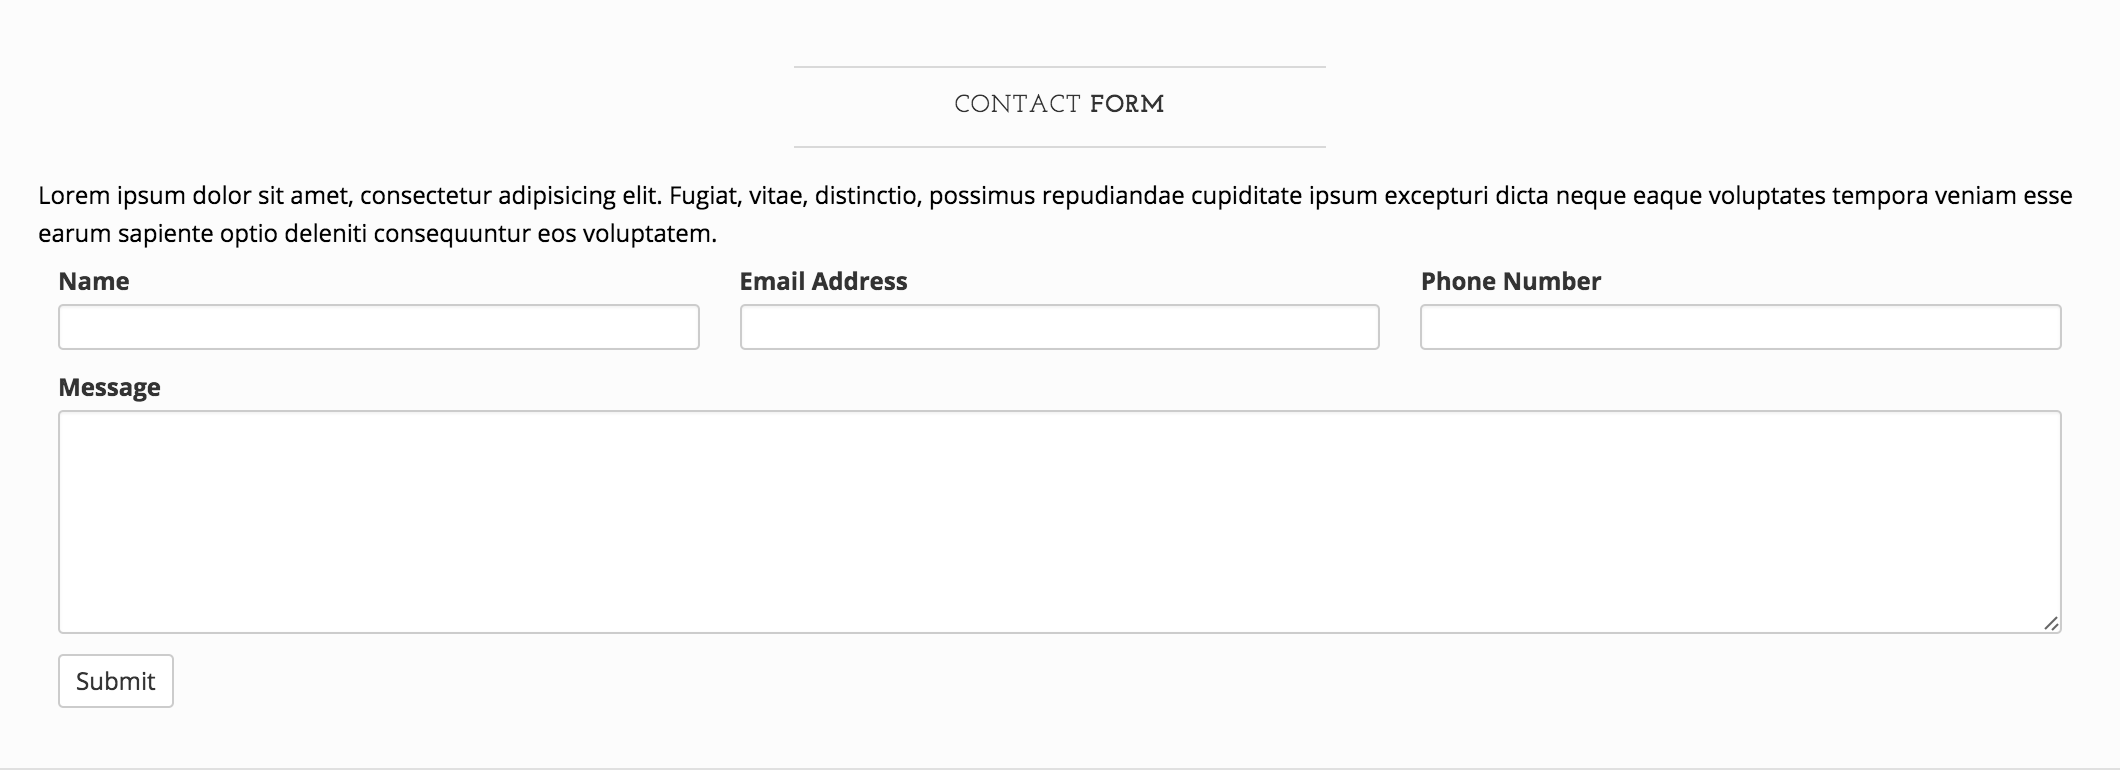
\includegraphics[width=17cm, height=5cm]{email.png}

\subsection{Android Application Viewport Redirection}
\begin{lstlisting}[language=java]
...
@Override
    public boolean shouldOverrideUrlLoading(WebView view, String url) {
        if (Uri.parse(url).getHost().endsWith("healthcareersoregon.com")) {
            return false;
        }
...
...
 // Enable Javascript
        WebSettings webSettings = mWebView.getSettings();
        webSettings.setJavaScriptEnabled(true);

        // Use remote resource
        mWebView.loadUrl("healthcareersoregon.com");
...
\end{lstlisting}
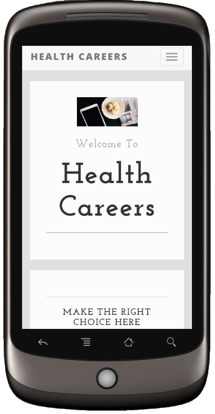
\includegraphics[width=5cm, height=10cm]{phone.png}
\newpage
\noindent In importData.php, one of the important coding segments is connecting into the database. In order to gain access the data from the database the dbConfig.php must be included at the top of the file. 
\subsection{Database Connection Variables}
\begin{lstlisting}[language=PHP]
<?php
	//load the database configuration file
	include 'dbConfig.php';
\end{lstlisting}

\noindent dbConfig.php consist of five variables that verify the connection for database. This part of code is being mentioned in the Usage and Maintain Guide session. 

\begin{lstlisting}[language=PHP]
<?php
//DB details
$dbHost = 'xxxx';
$dbUsername = 'xxxx';
$dbPassword = 'xxxx';
$dbName = 'xxxx';

//Create connection and select DB
$db = new mysqli($dbHost, $dbUsername, $dbPassword, $dbName);

if ($db->connect_error) {
    die("Unable to connect database: " . $db->connect_error);
}
\end{lstlisting}

\noindent It is important to ensure that the functionality to upload spreadsheet is valid. The only type of file that can be used to upload data to our database is a CSV spreadsheet. A comma-delimited CSV file can be parsed into variables to upload to the database.
\subsection{File Parsing}
\begin{lstlisting}[language=PHP]
//validate whether uploaded file is a csv file
    $csvMimes = array('text/x-comma-separated-values', 'text/comma-	separated-values', 'application/octet-stream', 'application/vnd.ms-excel', 
    'application/x-csv', 'text/x-csv', 'text/csv', 'application/csv', 'application/excel', 'application/vnd.msexcel', 'text/plain');
    if(!empty($_FILES['file']['name']) && in_array($_FILES['file']['type'],$csvMimes)){
        if(is_uploaded_file($_FILES['file']['tmp_name'])){
            
            //open uploaded csv file with read only mode
            $csvFile = fopen($_FILES['file']['tmp_name'], 'r');
            
            //skip first line
            fgetcsv($csvFile);
\end{lstlisting}

\noindent If the tables exist and error-free, then execute the queries using SQL based on your desire. The SQL can retrieve, insert, update, delete, or create records within the database. 
\subsection{Uploading to Database}
\begin{lstlisting}[language=PHP]
if($prevResult->num_rows > 0){
//update member data
$db->query("UPDATE Careers SET careerID = '".$line[0]."',
careerName = '".$line[1]."', entryEdu = '".$line[2]."',
compEdu = '".$line[3]."', category = '".$line[4]."', 
statistics = '".$line[5]."', bodyText = '".$line[6]."',
img = '".$line[7]."', caption = '".$line[8]."'
WHERE careerID = '".$line[0]."' ");
}
else{
   ...
}
\end{lstlisting}

\newpage
\section{Appendix 2: Additional Images}
\vspace{.8cm}
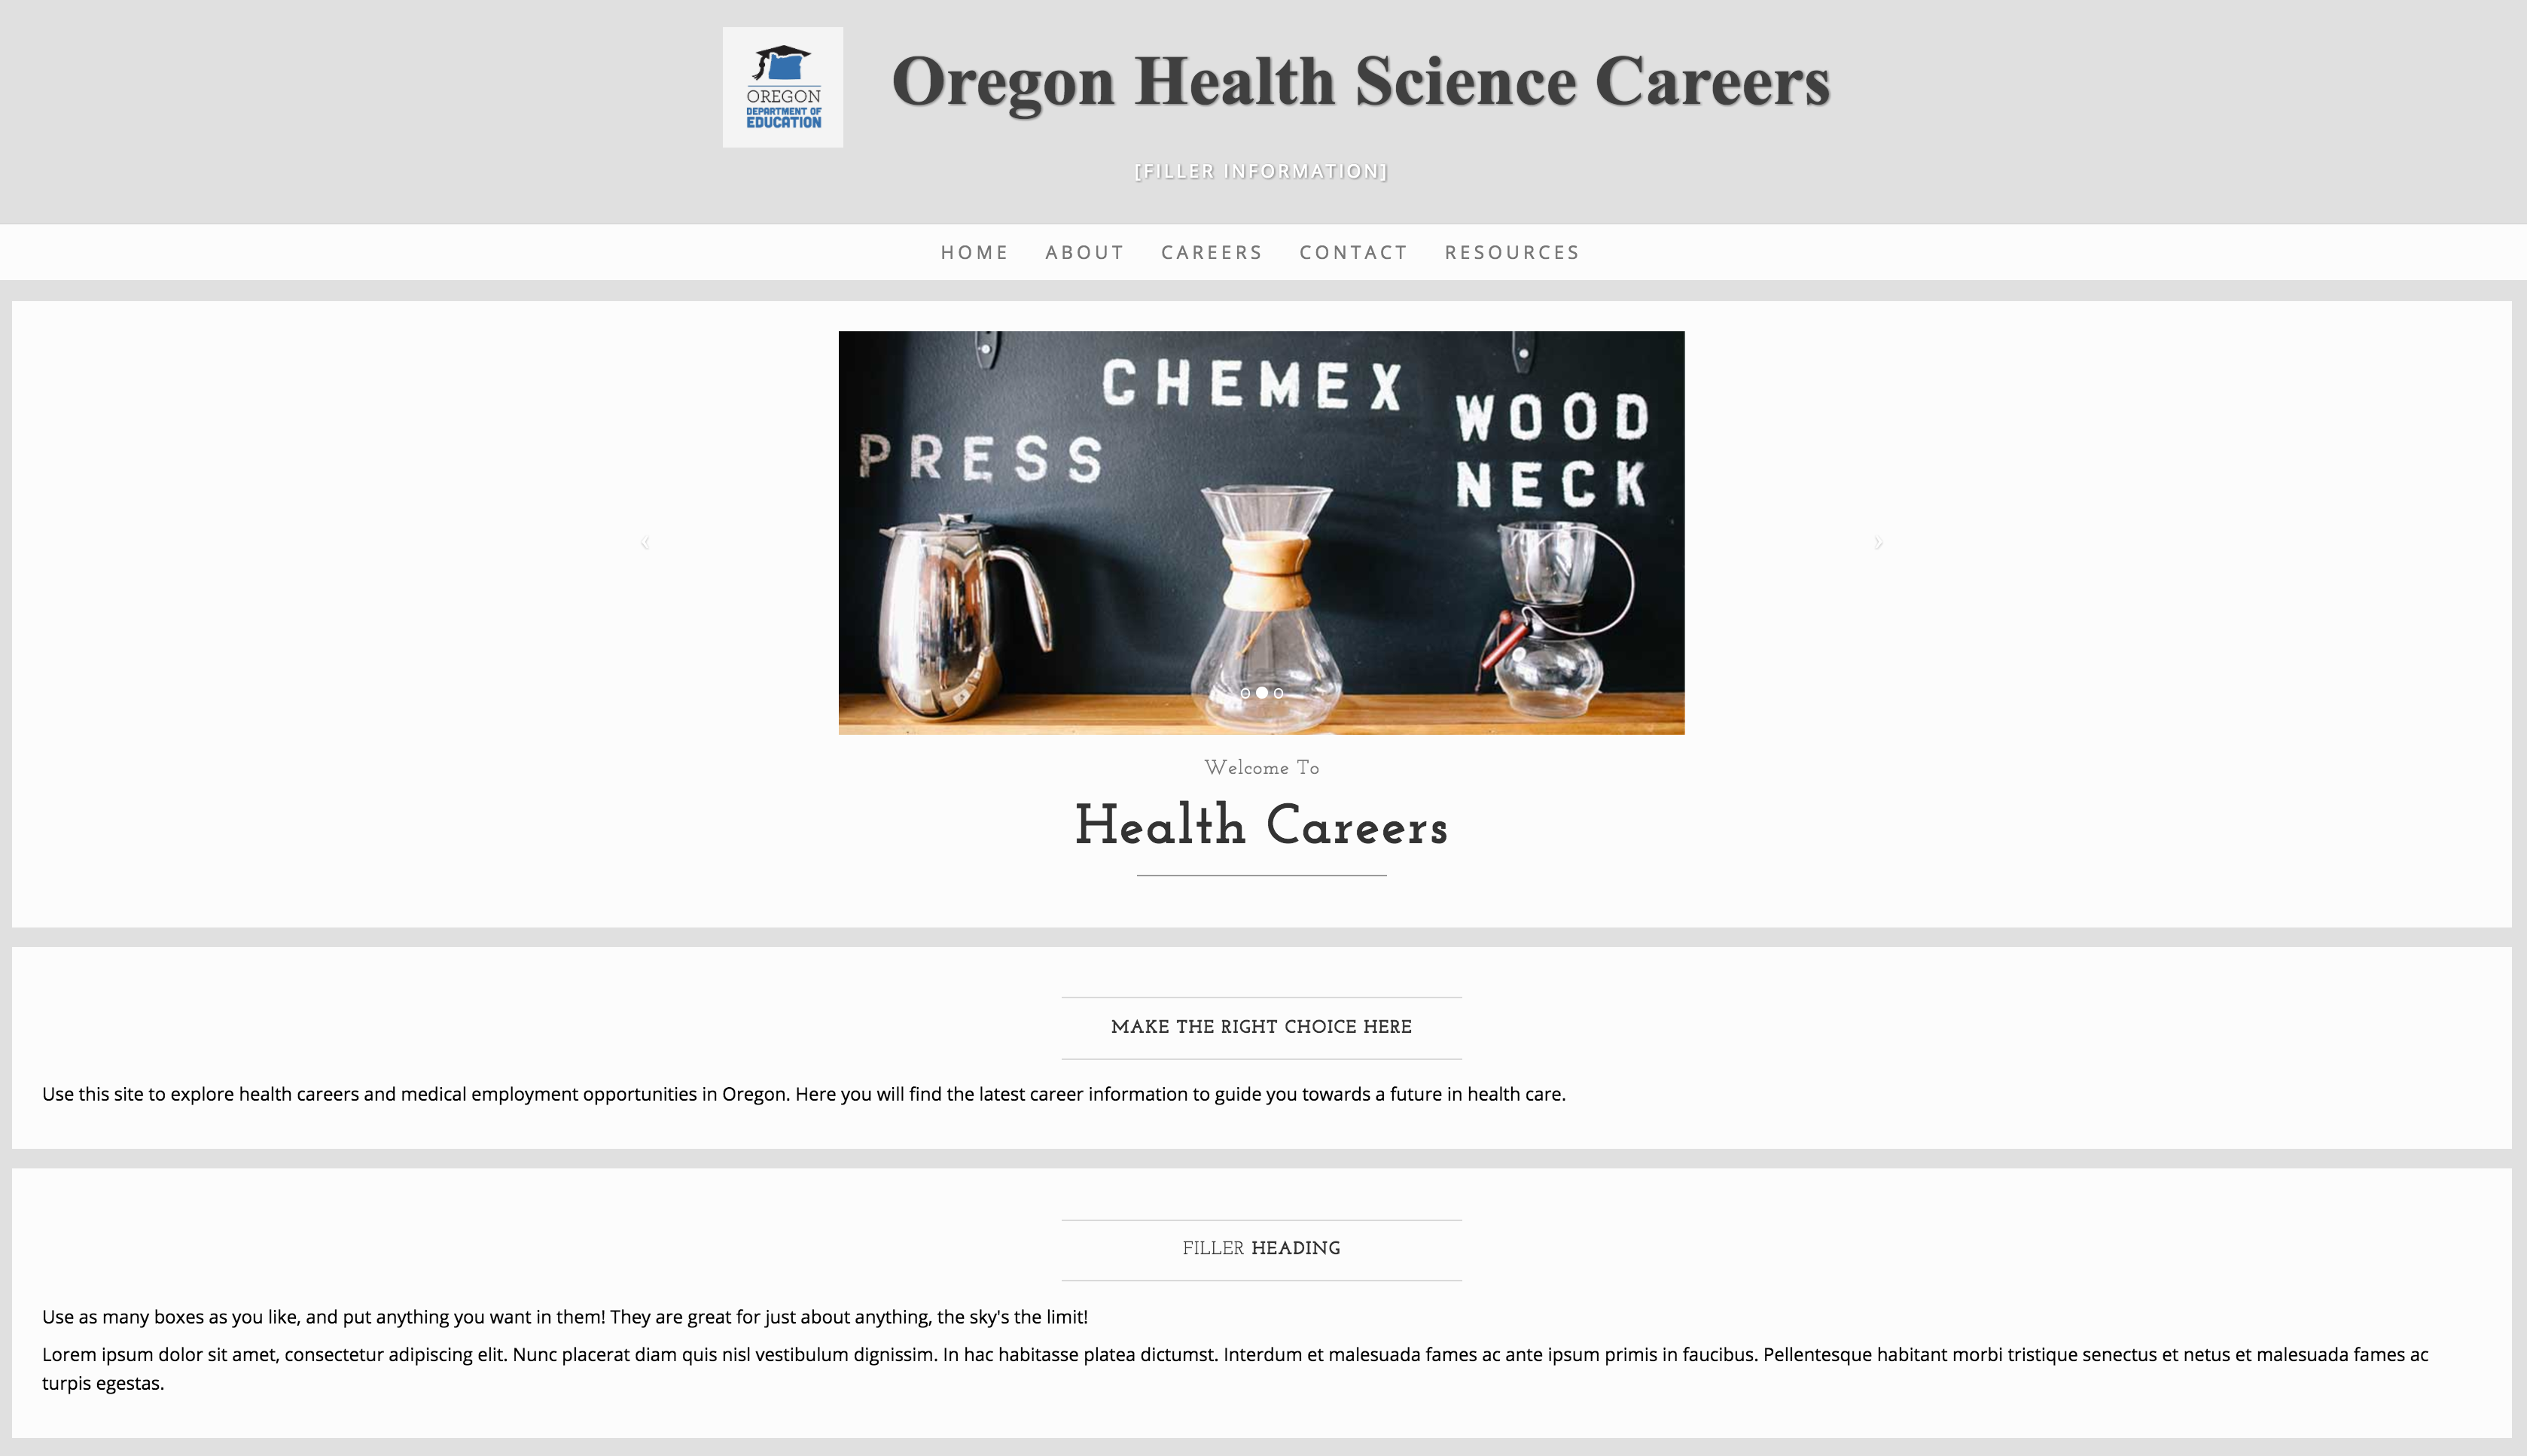
\includegraphics[width=16.78cm, height=9.67cm]{webiste1.png}
\\ \\
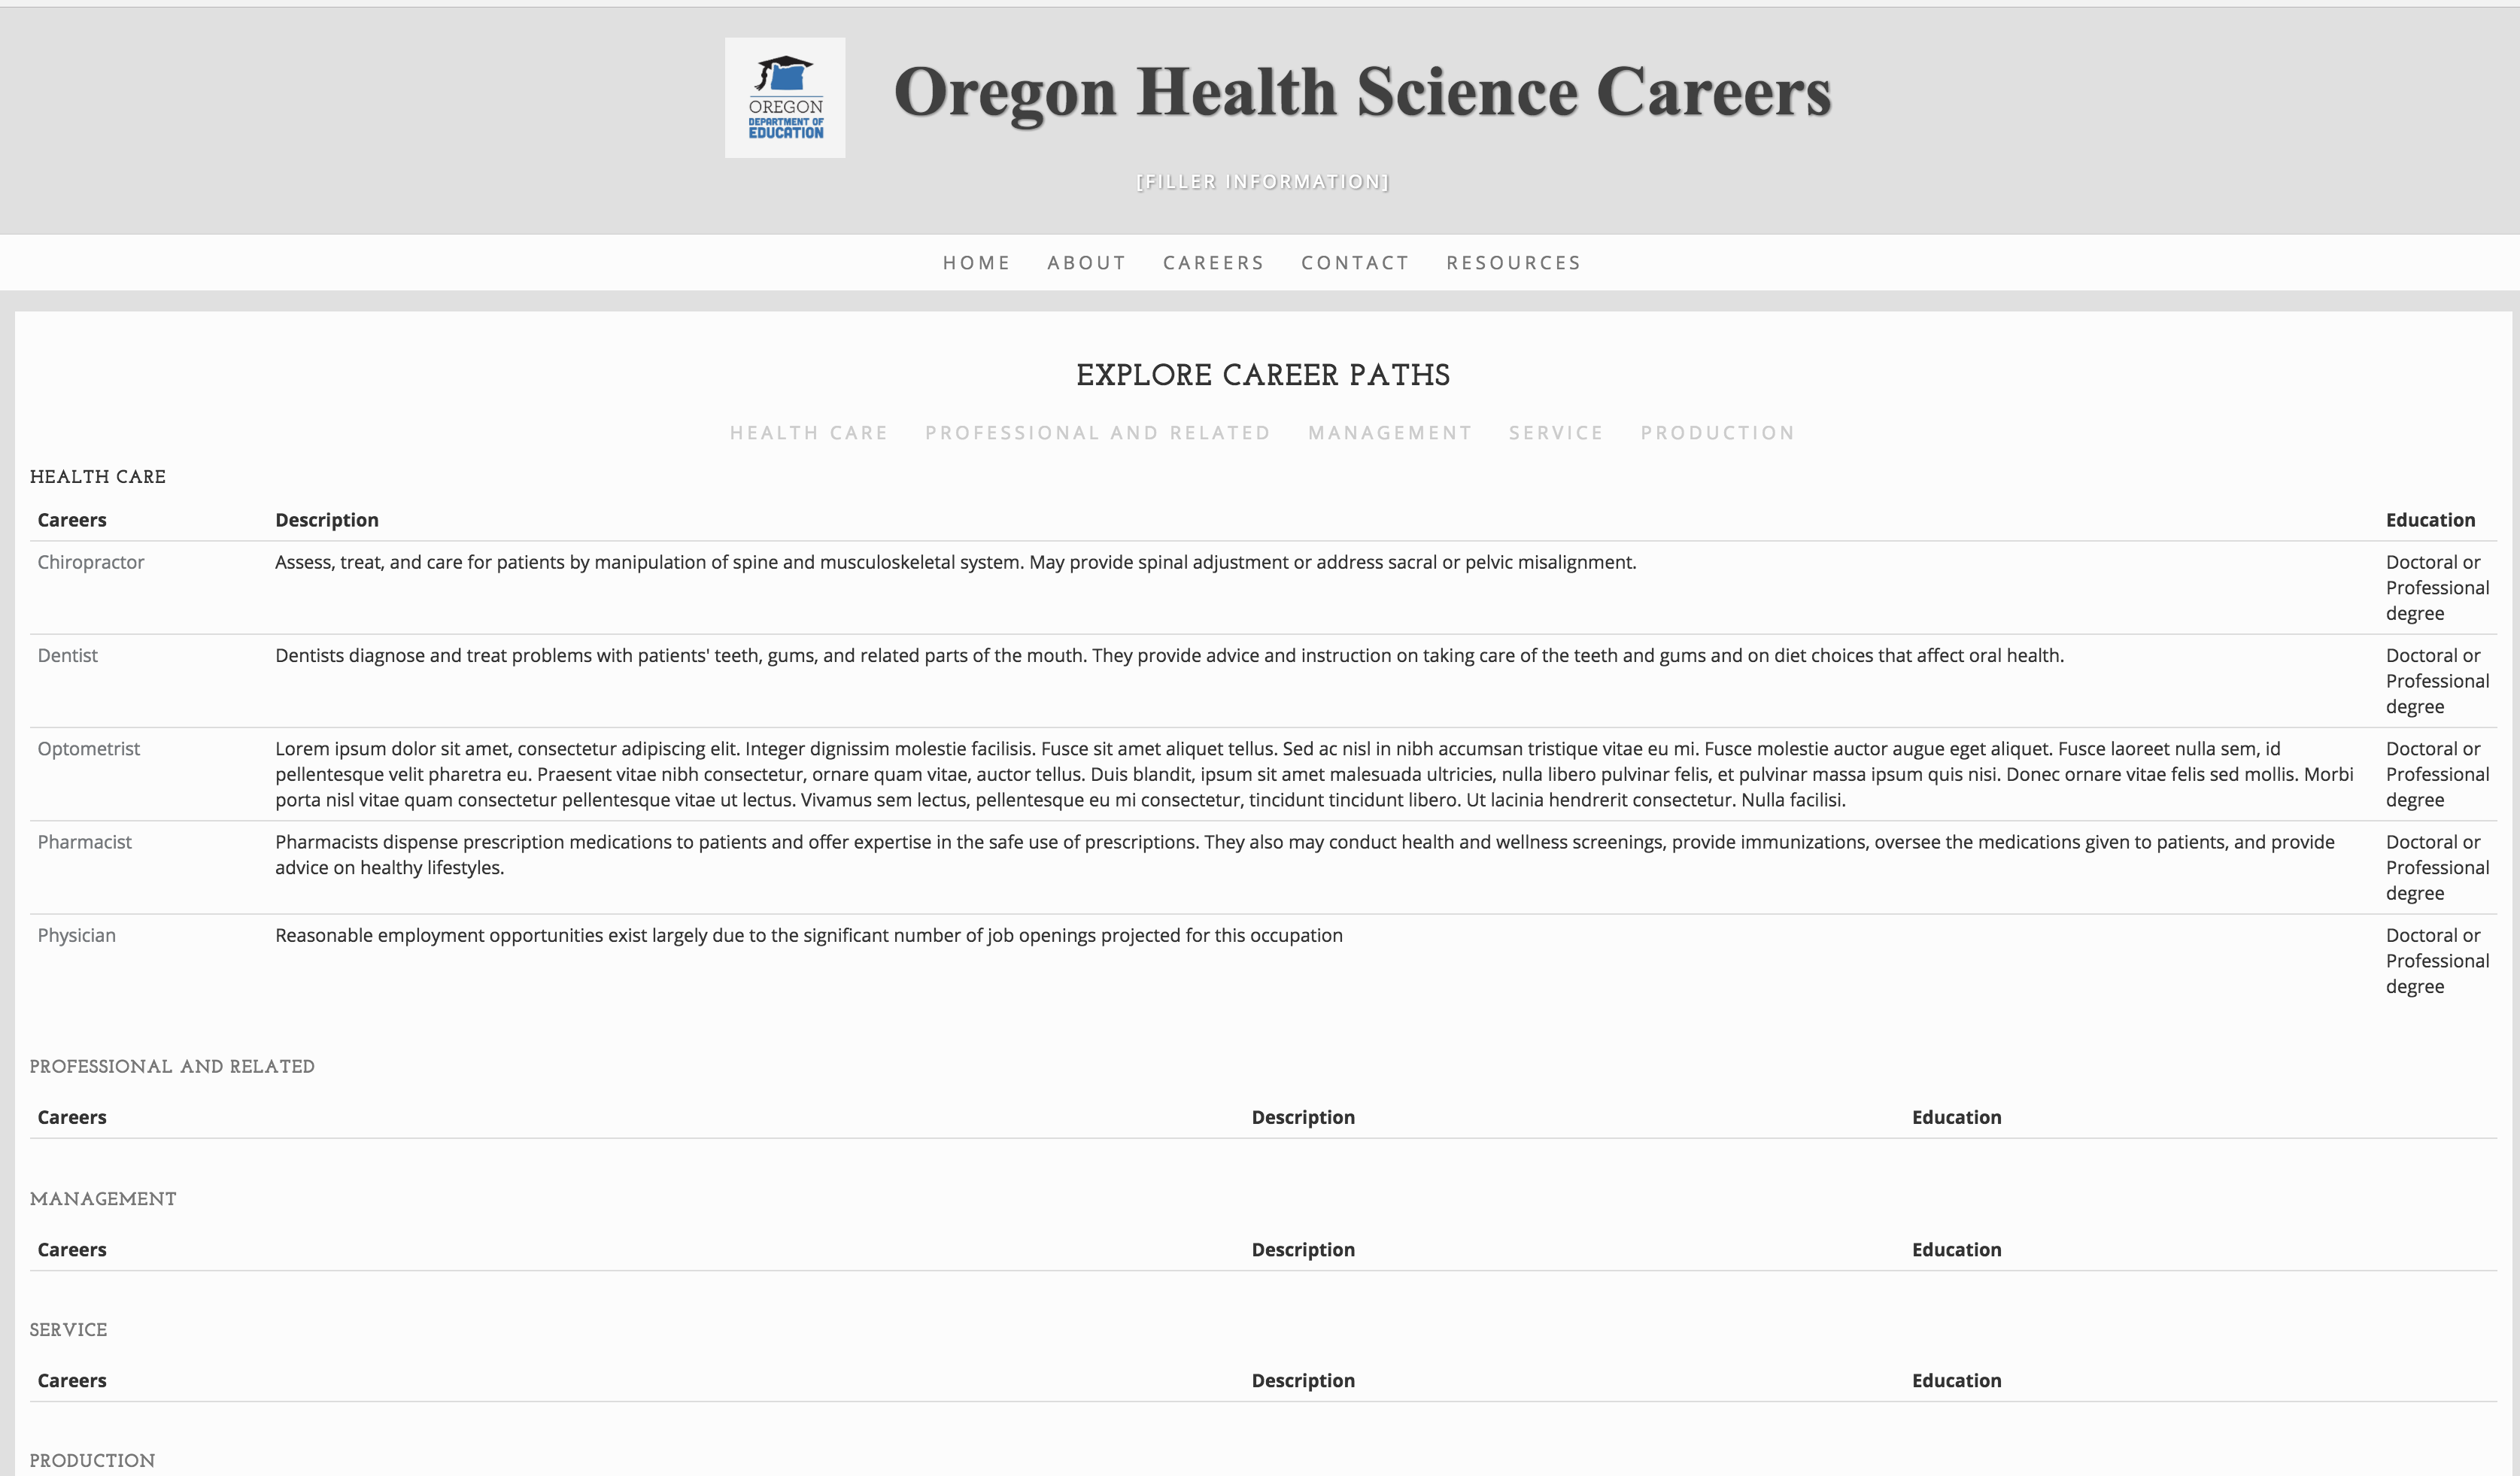
\includegraphics[width=16.78cm, height=9.67cm]{webiste2.png}
\\ \\
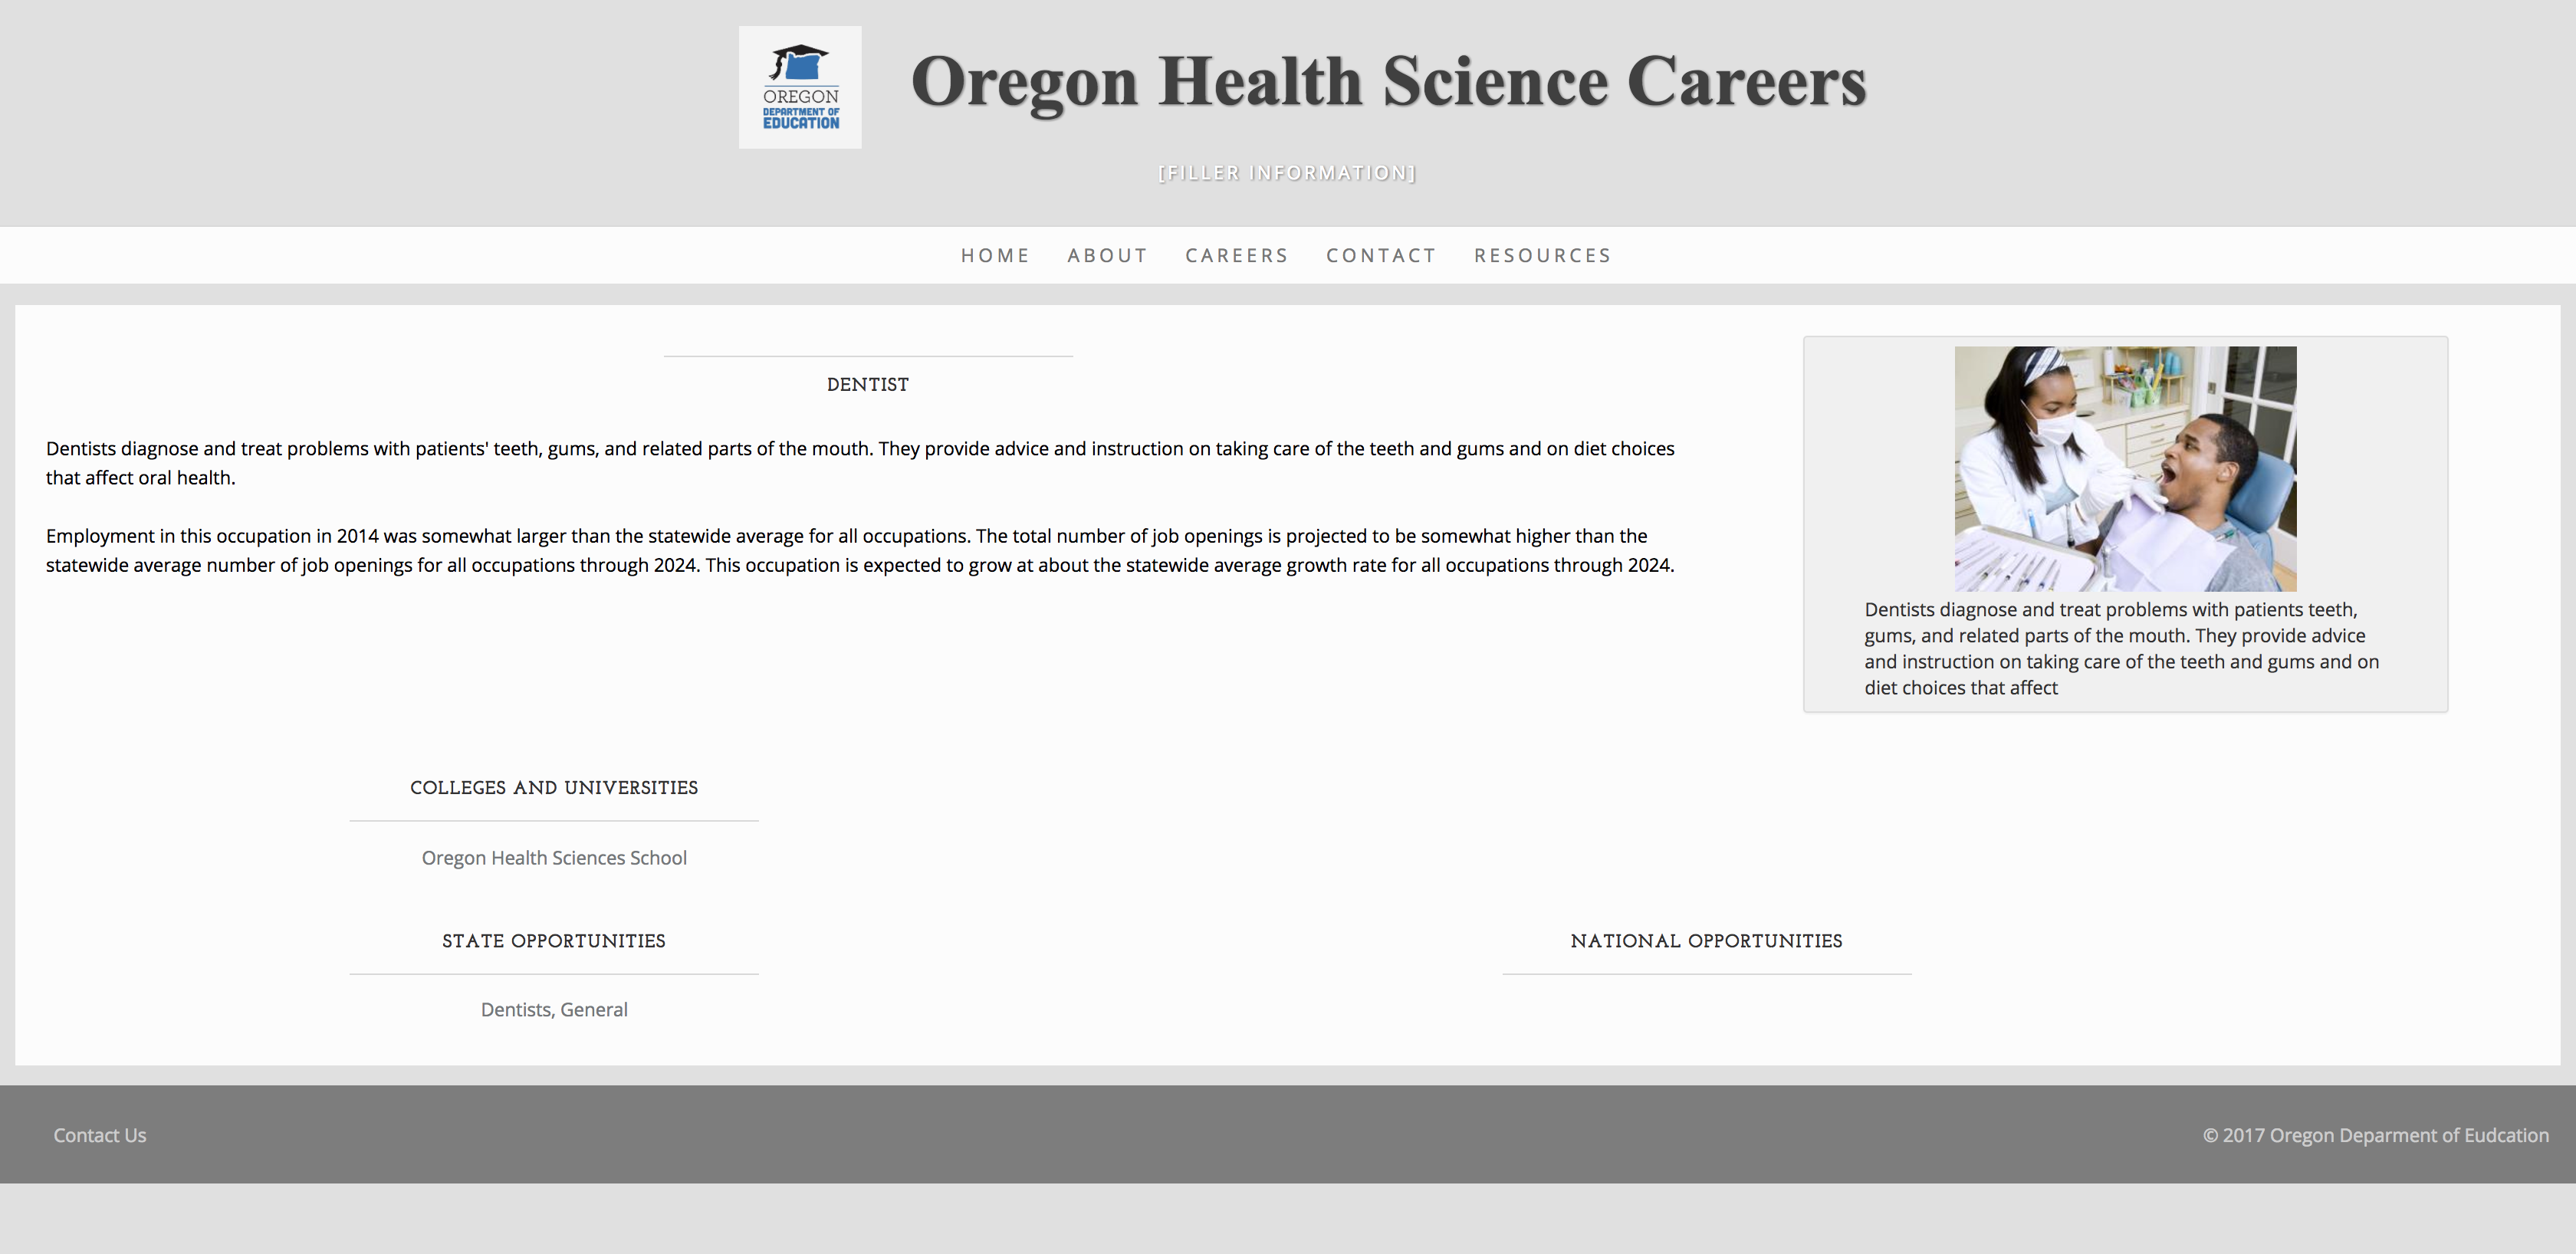
\includegraphics[width=16.78cm, height=9.67cm]{website3.png}
\\ \\
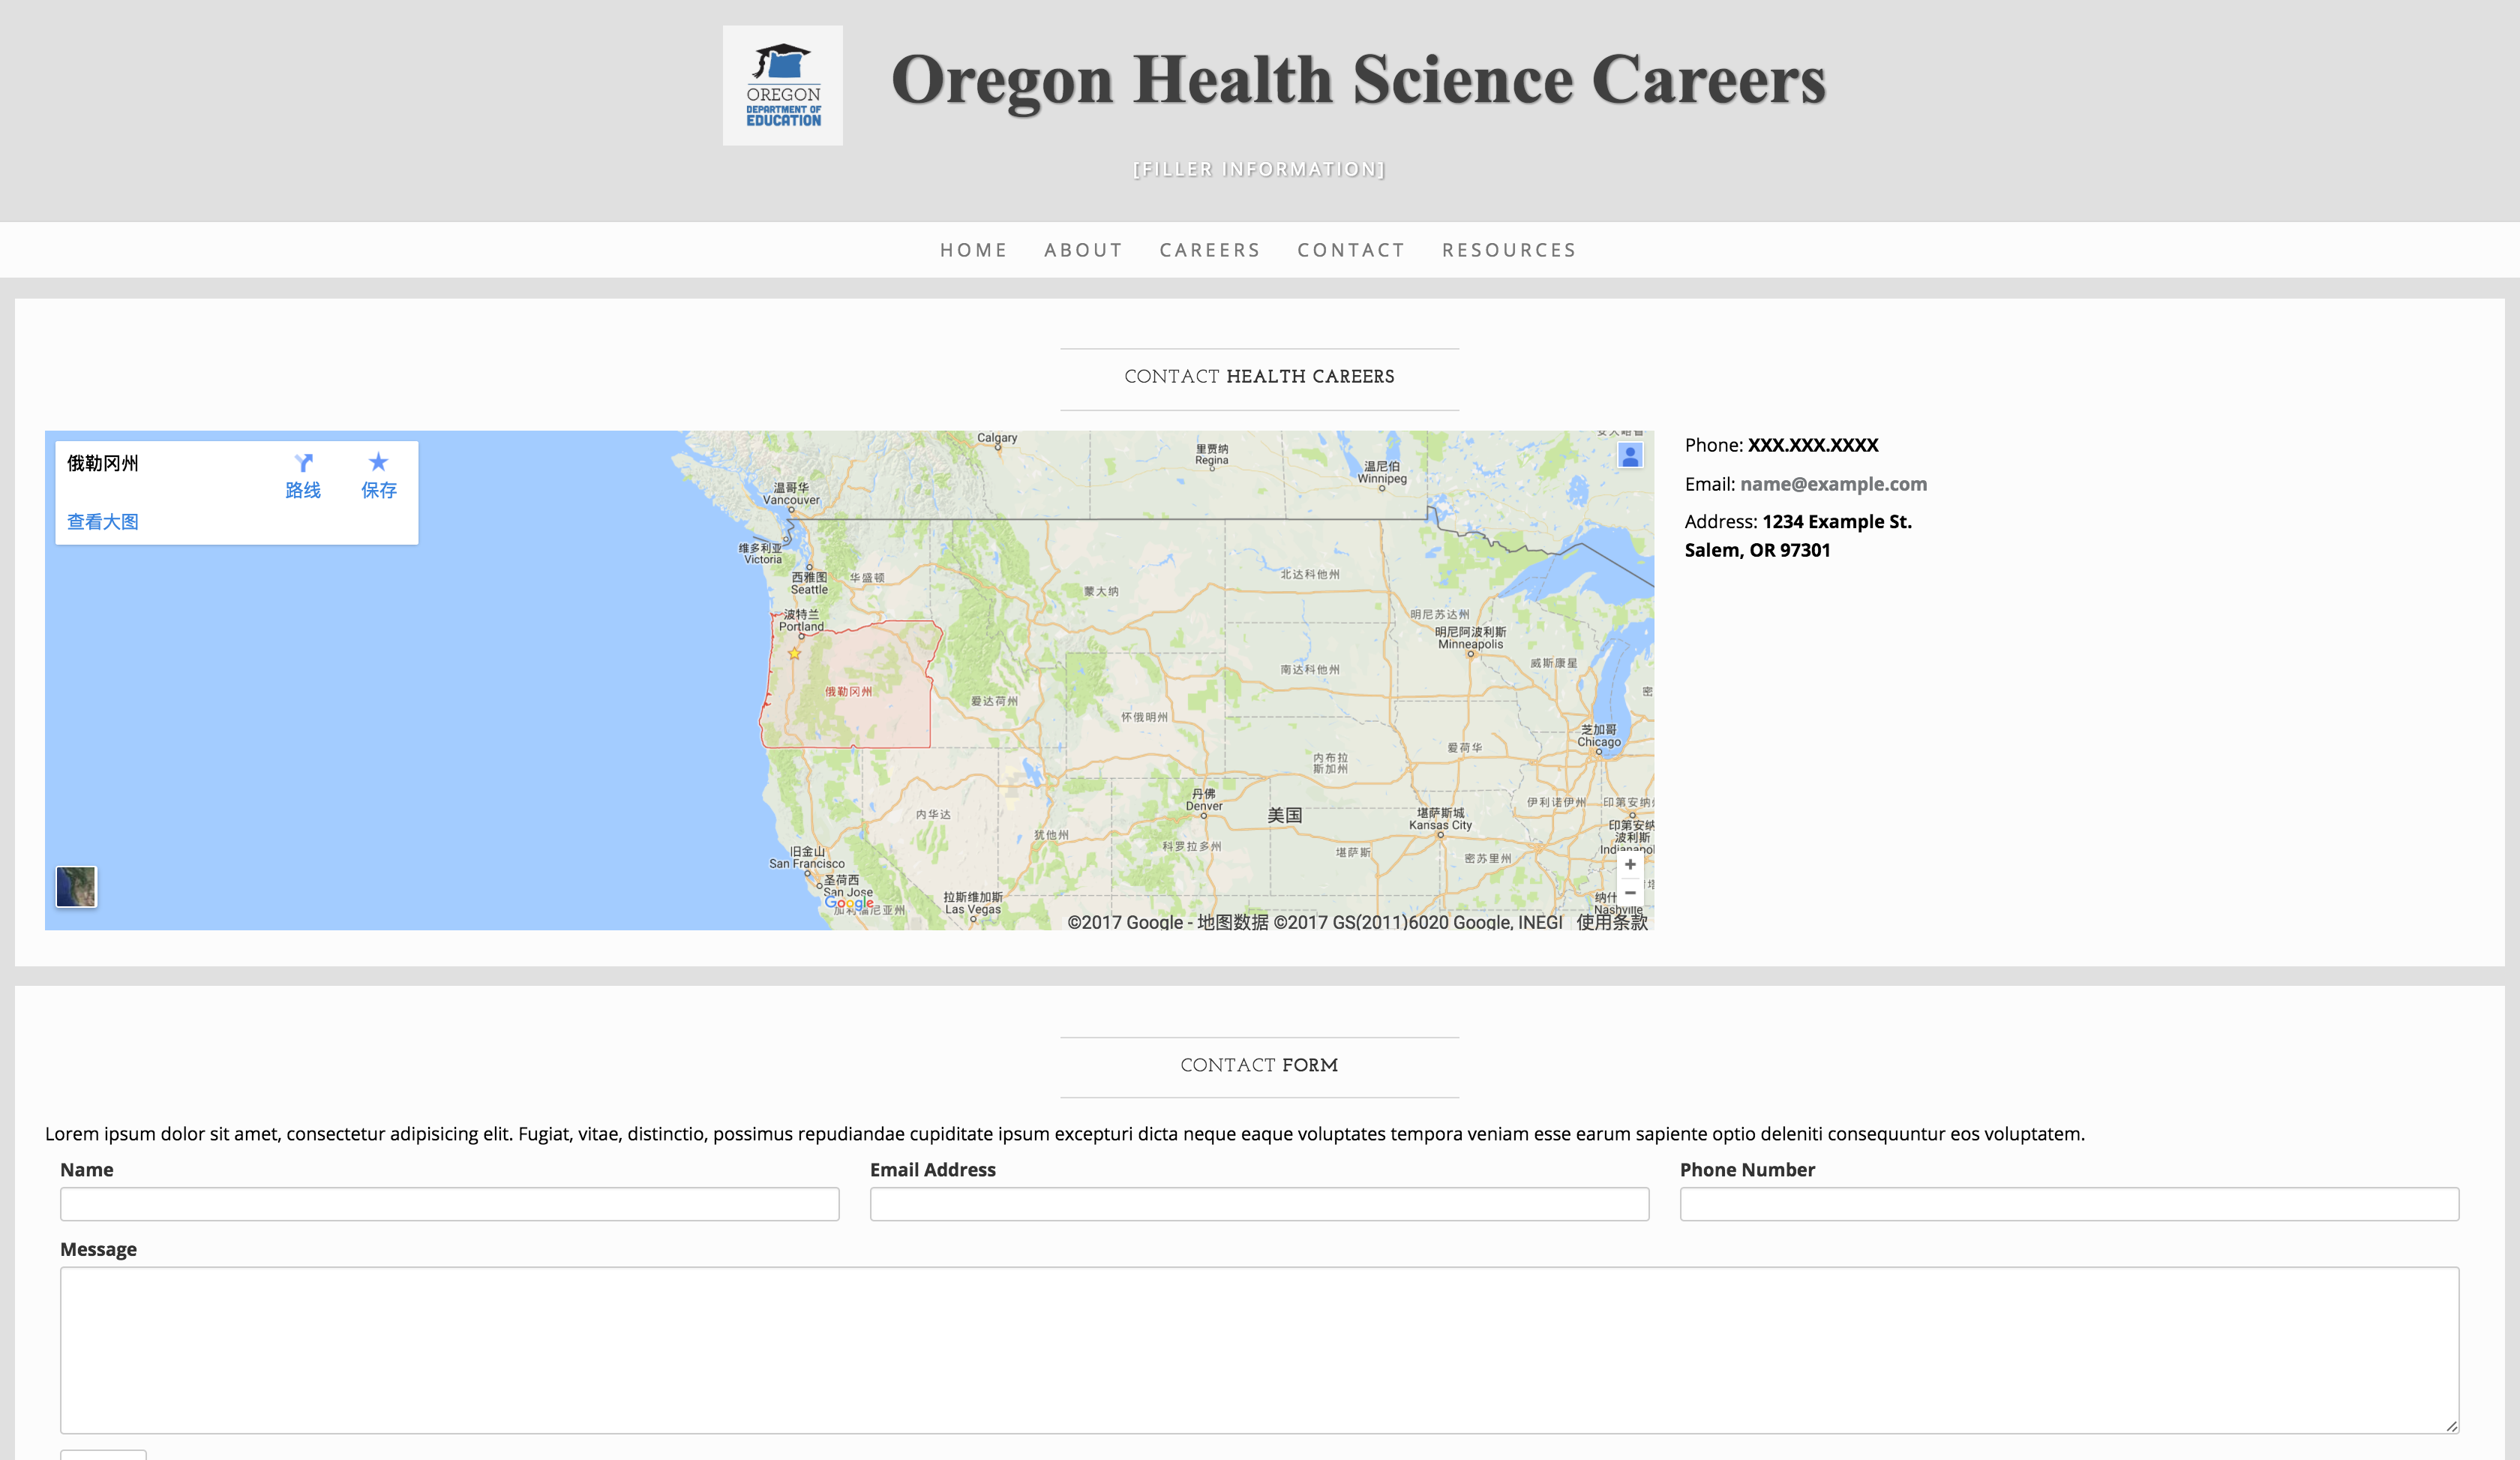
\includegraphics[width=16.78cm, height=9.67cm]{website4.png}
\\ \\
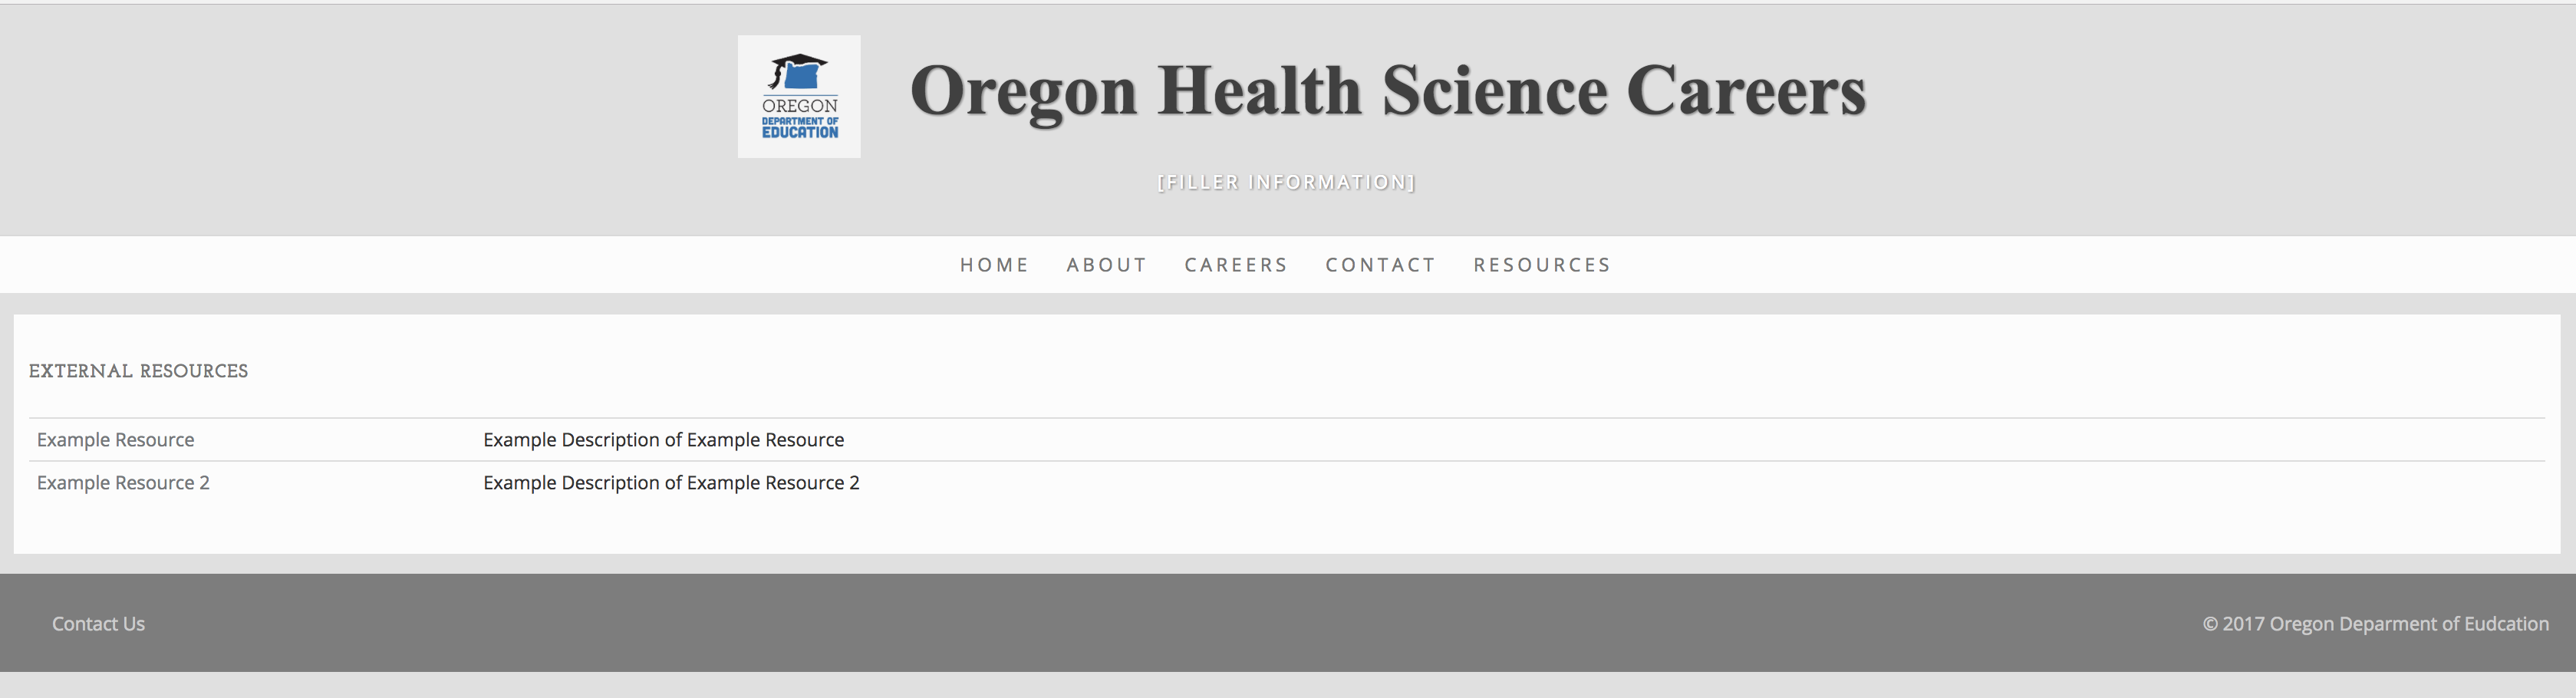
\includegraphics[width=16.78cm, height=6cm]{webiste5.png}
\\ \\
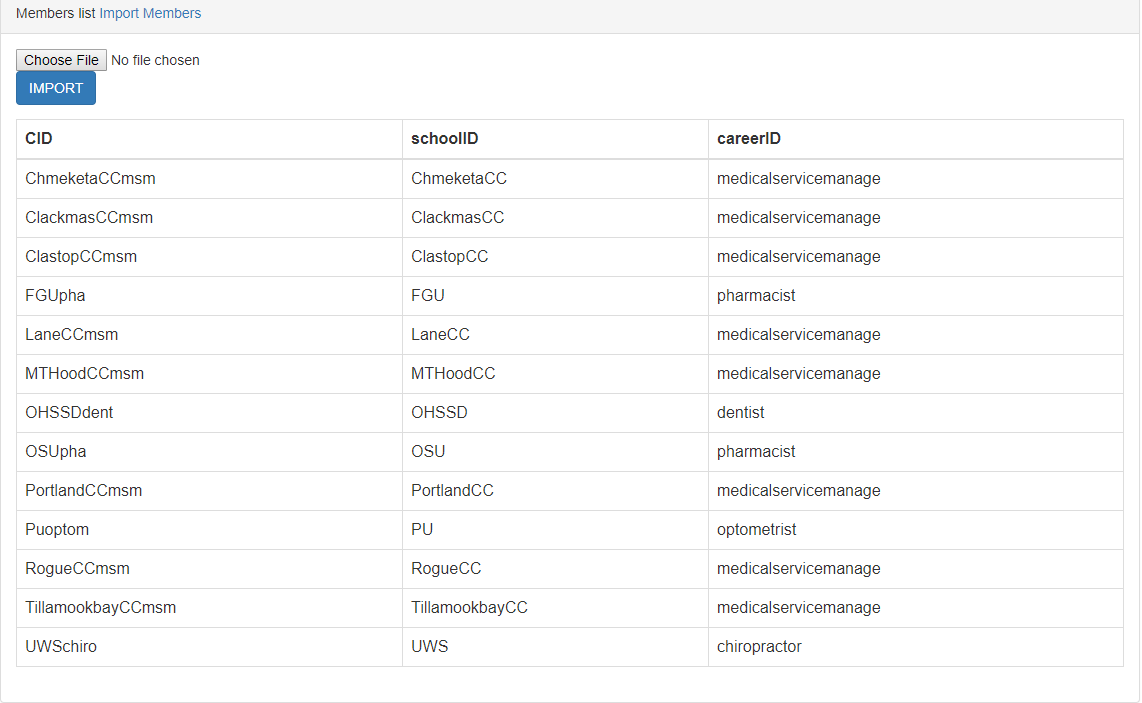
\includegraphics[width=16.78cm, height=9.67cm]{DataUpload.png}
\\ \\
\end{document}